
\chapter{Blockchain Technology in Games}
\label{chap:BlockchainInGames}
Since \citet{Nakamoto.2009}'s paper, many different \gls{CM}s were invented,
as given in section \hyperref[sec:ConsensusMechanisms]{Consensus Mechanisms}.
Currently the use cases of \gls{BCT} in games can be grouped by concepts of 'real-world ownership',
'digital tokens which represent game assets', the 'reduction of upkeep costs' as well as 'enhanced engagement from the user-base' \cite[15]{Laneve.2019}.
In other words, \citet[1]{Min.2019} state that \gls{BCT} in games is used for \textit{Rule Transparency},
\textit{Asset Ownership}, \textit{Assets Reusability}, \textit{User-Generated Content} as well as  \textit{Current scalability}.
Therefore, using ".. games to grasp the functionalities of cryptocurrencies and the blockchain technologies that make them possible seems like an obvious choice"
\cite[2]{Serada.2020}, especially as beneficial synergies between the needs of gaming networks and promises of \gls{BCT} can be found.
This intersection seems to be situated around slow paced asynchronous games, as \gls{BCT} is basically not suited for fast applications \cite[19]{Serada.2020}.
Therefore the following chapter wants to answer the first guiding question:
\textit{"Which kind of \gls{SC}s need to be established to cover typical in-game mechanics?"}. \\
Hence, \textbf{first} recent solutions are analyzed and grouped by \textit{ownership}, \textit{gameplay} and \textit{network costs}.
\textbf{Second}, the gaming market is examined briefly and some sample games are presented.
This shows blind spots of \gls{BCT} game play and respective (asynchronous) in-game mechanics.
\textbf{Third}, a problem area is defined to increase tangibility of problems in distributed games.
\textbf{Last} some solutions to these problems are shown, custom tailored for distributed game play. \\
Afterwards, assuming that \gls{BCT} is suitable for (asynchronous) games, the following chapter,
\hyperref[chap:PoT]{Proof-of-Turn}, will provide a \gls{CM} which aims to deliver
the features described at the end of the last chapter, \hyperref[chap:BCT]{Blockchain Technology}.

\section{Ownership,  network costs, gameplay \& scalability}
\label{sec:OwnershipGameplayNetwork}
For \textbf{ownership} models, the general idea is derived from Bitcoin which administers a cryptocurrency.
Besides or instead of a cryptocurrency, digital assets are regulated by the game's \gls{BC} \cite[2]{Pfeiffer.2020}.
This idea is called \textit{Collectibles (Collection Games)} and, as it is not too circuitous,
it was one of the first mentioned type of games hosted on \gls{BCT}.
"The ownership enables the game assets to be independent of specific game operators, which allow the players to retain their digital properties and in-game relationships, even after the game stops its operation" \cite[1]{Min.2019}.
A prominent example is \textit{CryptoKitties} \cite[2]{Pfeiffer.2020}.
Next to CryptoKitties many other cryptogames were developed (e.g., Cryptopunks, Decentraland, MyCryptoHeroes, HyperDragons, Gods Unchained, Etheremon, Blockchain Cuties, NeoWorld, and Axie Infinity) \cite[2]{Serada.2020}, which fall into this category.
A sample store to buy assets from these \textit{Collectibles} might look like figure \ref{fig:Collectibles}.
Digital assets can be bought using some sort of payment channel (here the cryptocurrency: \gls{ETH}).
Sometimes \textit{Collectibles} offer the opportunity to breed new assets out of the existing ones \cite[2]{Serada.2020}.
During breeding properties (here: border thickness, colors, edges, size etc.) of two shapes are recombined.
To increase asset diversity, sometimes mutations happen and new characteristics (e.g. color gradients, figure \ref{fig:Collectibles}: rectangle) occur, which makes the single asset special.
As a bread shape can be considered a child-generation of the two parent shapes, breeding generations are given (compare \cite{CryptoKitties.co.2021}).
The breeding may be rather seen as part of the \textit{Collectibles}-game than part of the asset ownership itself \cite[2]{Pfeiffer.2020}.
Further, one advantage of \textit{Collectibles} is, that the "[...] possibility of asset trades across different games and blockchain platforms stimulates the players to better engage in the game economy" \cite[1]{Min.2019}.
Regarding \textit{reusability}, game "[...] developers can leverage blockchain to design an ecosystem that allows players to reuse their characters and virtual items across different games.
\begin{figure}
	\centering{
		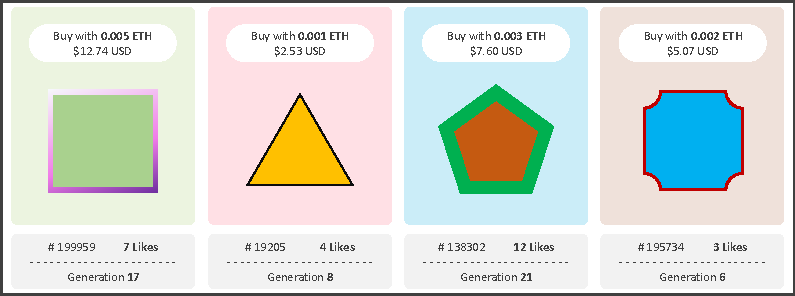
\includegraphics[width=.95\linewidth,keepaspectratio=true]{contents/images/Collectibles}
		\caption{Collectibles store 'CryptoShapes' (Adapted from \citet{CryptoKitties.co.2021})}
		\label{fig:Collectibles}
	}
\end{figure}
To this end, newly launched games can directly inherit game assets from the existing ones" \cite[1]{Min.2019}. \\
Moreover, User-Generated Contents "[...] in traditional games are restricted in the specific game, thus, belongs to the game operator.
In contrast, these contents can be preserved by the players, thus, has the potential to be shared among multiple games.
This benefit will, in turn, encourage the players to participate in the construction of new content"
\cite[1]{Min.2019}. \\
These connected games are called 'Layer two games' as they use \gls{NFTs} "[...] from other games to fuel their gameplay.
Players could only access these games by using items they had acquired from other sources" \cite[26]{Laneve.2019}.
Depending on the used cryptocurrencies or tokens, "[...] game operators may benefit from the value increase of the tokens they issued" \cite[1]{Min.2019}. \\

\noindent \textbf{Network costs} \textemdash \hspace{0.075cm} No game has been found which uses \gls{BCT}
only for the sake of reducing upkeep costs of servers, yet.
In this regard, \citet[3]{Serada.2020} states:
"Oftenmost cryptogames are neither developed by game companies nor is their
design shaped by typical business models or assumptions such as profit making." \\

\noindent \textbf{Gameplay} \textemdash \hspace{0.075cm}Here,
the literature emphasizes the value of \textit{rule transparency} as an anti-cheating mechanism and \gls{BCT}'s potential in games (\citet[57]{Dib.2018}; \citet[1]{Min.2019}).
\gls{BCT} "[...] addresses one of the biggest issues with direct peer-to-peer transactions online; that is, a lack of trust.
Historically, a lack of trust has been cited as one of the greatest disadvantages of online gambling [...]" \cite[483]{Gainsbury.2017}.
"Due to the transparent characteristic of blockchain data, players or third-party organizations can audit
the smart contract based games rules, which was hidden in the centralized server in traditional games.
The transparent game rules will enhance the trustworthy of the game operation" \cite[1]{Min.2019}. \\
Yet, except the theoretical \gls{PoP} paper from \citet{Yuen.2019}, the literature only shows one single example of \gls{BCT} in games to effectively replace the \textit{central server network approach} (\citet{Wu.2020}) especially if cryptocurrency ownership models are \textit{excluded}.
\citet[4559-4560]{Wu.2020} came to the same conclusion:
"To the best of our knowledge, this is the first blockchain-related game demostration that achieves a real-time serverless gaming system with an anti-cheating mechanism."
Still no professionally produced game could be found, which already left its BETA-status or
can be considered more than a proof of concept, such as \textit{Huntercoin} (\citet{Kraft.2016}). \\


\noindent \textbf{Current scalability} \textemdash \hspace{0.075cm}Additionally, scalability of BCT has to be put in contrast:
"As it stands, blockchain technology does not seem applicable for the design of the most popular game genres such as first-person shooters or real-time strategy, although several attempts have been made in this direction [...]" \cite[3]{Serada.2020}.
\begin{figure}[!b]
	\centering{
		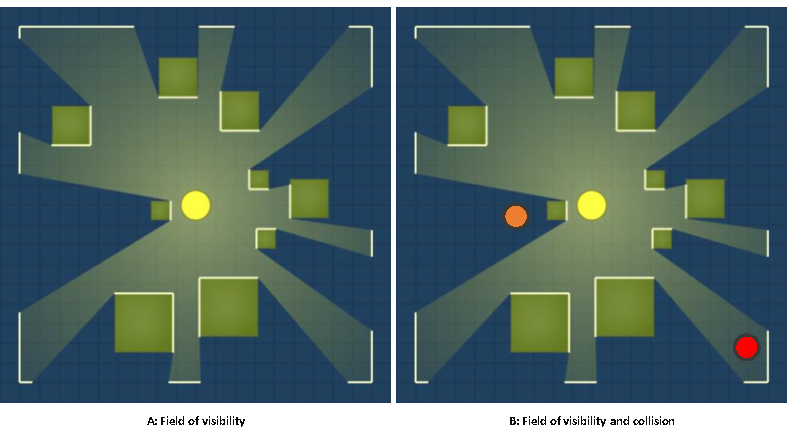
\includegraphics[width=.95\linewidth,keepaspectratio=true]{contents/images/VisibilityScalability}
		\caption{Visibility and Scalability}
		\label{fig:VisibilityScalability}
	}
\end{figure}
This statement derives from \gls{BCT} focusing on consistency and partition tolerance regarding the CAP-Theorem instead of high availability (\citet{Angelis.2018}).
Additionally cryptocurrencies like Ethereum and Bitcoin show that "read availability of blockchains is typically high [...]"
whilst "[...] write availability — for transaction management — is actually low" \cite[64]{Weber.2017}. \\
Furthermore, in a centralized server context, all players ($p$) send their information to the
server - 'one on one' relationships for the players and 'one to $p$' for the server, sum: $2p$.
In \gls{CM}s wherein all nodes are allowed to write, the number of relationships ($r$) becomes squared ($r = p^2$).
Consequently, consultation and throughput increases tremendously with growing networks.
\gls{CM}s which reduce the writing nodes, help to cure this scalability issue. \\
Additionally, a major constraint is the visibility of every player.
It has to be determined who receives necessary (movement) information and who does not.
This could either be done to hide information or to reduce network throughput.
This information is especially restricted by objects blocking the visibility as shown in the 2D-figure \ref{fig:VisibilityScalability} (Playground of \citet{RedBlobGames.2020} was used).
In figure \ref{fig:VisibilityScalability}, a player (circle, middle) is shown with its range of visibility (lighted area).
The visibility is blocked by rectangular objects, which cast shadows.
Yet alone in figure \ref{fig:VisibilityScalability} (A) there are no constraints.
But assuming other players around (Figure \ref{fig:VisibilityScalability}, B) one can tell that distance is not the only measure for other players to be displayed - a 'Line of Sight' has to exist.
Leaving the display to honest nodes is not applicable here as fraud is a major concern in this document.
Adding cryptography and signing information only to specific players to prevent fraud, slows down the network even more.
Consequently, whilst a fast paced four player game might be possible using the right \gls{CM},
40 simultaneous players as in \textit{Star wars Battlefront} (\cite{Wikipedia.2021e})
or even 64 as in \textit{Battlefield} (\cite{Wikipedia.2021}) are far out of reach \cite[3]{Serada.2020}. \\
Last, in distributed environments each player wants to keep its position secret as long as possible to prevent cheating.
Still the position of both players has to be published to calculate the possibility of a 'line of sight'.
This brings the anti-cheat mechanism at odds.
Hence, \gls{BCT} is clearly not a solution for high traffic (shooter) games and
due \gls{BCT}s characteristic to be "barely scalable" \citet[19]{Serada.2020},
\gls{MMORPG}s with multiple simultaneous actions are out of scope as well.



\FloatBarrier

\section{Gaming market}
\label{sec:GamingMarket}

Until now the focus of the document was primarily on the technical side.
This section sheds the light on the recent gaming market - especially on the gamers.
The following data is taken from a market report of \citet{LimelightNetworks.2020}. \\
\textbf{First} it has to be determined which kind of device is suitable for games based on \gls{BCT}.
The given data \cite[7]{LimelightNetworks.2020} attest mobile phones a superior position for gaming globally (Figure \ref{fig:GameingDeviceData}).
This claim is backed by the data of each observed country (Appendix - Figure \ref{fig:GameingDeviceDataTable}).
\begin{figure}
	\centering{
		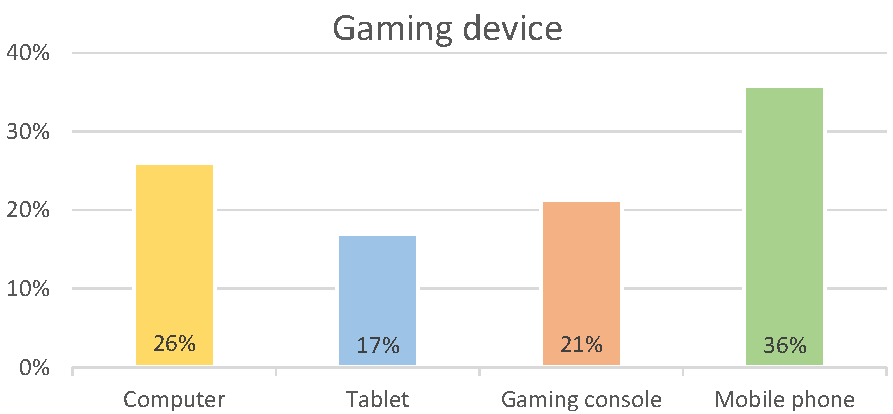
\includegraphics[width=.95\linewidth,keepaspectratio=true]{contents/images/GameingDevice}
		\caption{Global share of devices by gaming time (Data from \citet{LimelightNetworks.2020})}
		\label{fig:GameingDeviceData}
	}
\end{figure}
If a publisher wants to tackle a big market, mobile phones shall be considered before targeting personal computers and gaming consoles.
Additionally, tablets are also part of the mobile market as they are run with the same operating systems (\citet{statista.com.2021b}) and offer the same distribution channels.
Consequently, slow paced (turn based) games which can be played on mobile phones
or cross platform offer a market to be hosted on \gls{BCT}.
Although \hyperref[sec:DataAllocationImprovements]{data allocation improvements} may be established in a game,
\gls{BCT} still needs storage space \cite[81]{Besancon.2019} as data can not just be pulled on demand from a central server.
Still, as a \textit{Counterpoint Research}-article from \cite{Wang.2021} stresses:
"Average smartphone nand flash capacity crossed the 100GB threshold in 2020"
(Appendix: Figure \ref{fig:GameingDeviceStorageSpace}).
This trend enables gaming with smartphones using \gls{BCT}.
The other devices, \textit{computers} and \textit{gaming consoles}, from figure \ref{fig:GameingDeviceData} are supposed to offer more or at least similar amounts of storage capacity. \\
\textbf{Second}, game characteristics shall be mentioned which are preferred by gamers.
Data out of the report \cite[18]{LimelightNetworks.2020} offers five categories of preferred games (Appendix:
Figure \ref{fig:GameCharacteristicsDataTable}).
\begin{figure}[!b]
	\centering{
		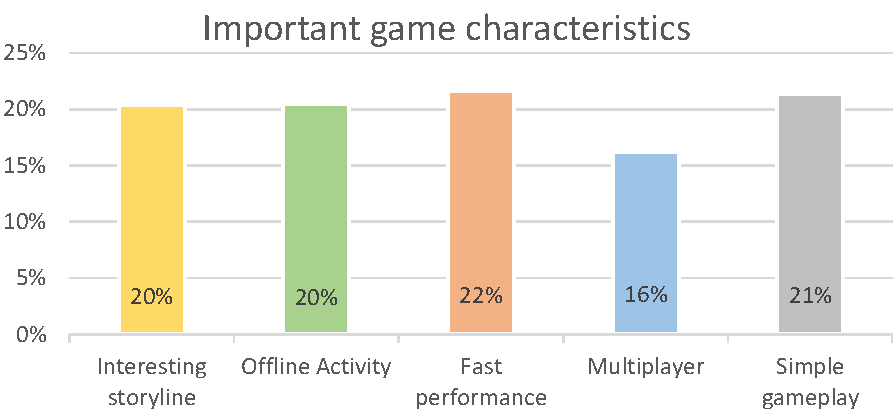
\includegraphics[width=.95\linewidth,keepaspectratio=true]{contents/images/GameCharacteristics}
		\caption{Global preferred game characteristics (Data from \citet{LimelightNetworks.2020})}
		\label{fig:GameCharacteristics}
	}
\end{figure}
The average of each category is shown in Figure \ref{fig:GameCharacteristics}.
The categories '\textit{Interesting storyline}' as well as '\textit{simple gameplay}' are out of scope as 
they have no influence on the game's backbone (e.g. \gls{BCT}).
On the contrary '\textit{Fast performance}', quickly loading and speedy interactions, '\textit{offline activity}',
the ability "to play the game while disconnected from the internet") \cite[18]{LimelightNetworks.2020}
as well as the '\textit{mulitplayer}' option are of importance regarding \gls{BCT}.
Here, \gls{BCT} enables offline time slots \cite[8]{Nakamoto.2009} in multiplayer games without the need for a central server.
Depending on the application - as stated before - fast performance is dependent on the chosen \gls{CM}. \\
\textbf{Third}, "[...] fair play is essential to any game [...]" \cite[44]{Yan.2009} and thus cheating (playing against agreed rules) harms gameplay.
Hence \cite[2]{HAEBERLEN.2010} cites from \cite{McGraw.2010}: "Cheating in online games is an important problem
that affects game players and game operators alike".
Many centralized games suffer in their game experience from this type of hostile behavior.
Therefore some "games try to prevent modding (e.g., multiplayer games to avoid cheating)" \cite[2493]{Lee.2020}.
Others install anti-cheating systems like PunkBuster, Warden or Valve Anti-Cheat \cite[8]{HAEBERLEN.2010}.
"In addition to privacy concerns, this approach has led to an arms race between cheaters and game maintainers,
in which the former constantly release new cheats or variations of existing ones,
and the latter must struggle to keep their databases up to date" \cite[8]{HAEBERLEN.2010}.
In the end anti-cheat measures commonly annoy gamers and reduce gaming system's performance.
With these problems in mind, \gls{BCT} promotes itself, despite its lack of speed
and the multiple data allocation, to be used in slow paced online (multiplayer) games.



\FloatBarrier

\section{Existing games using Blockchain Technology}
\label{sec:GamesOnBCT}

With the knowledge of the previously given four
categories \hyperref[sec:OwnershipGameplayNetwork]{Ownership,  network costs, gameplay \& scalability} , some already existing games, using \gls{BCT} are described:
\begin{enumerate}
	\item As described before \textit{CryptoKitties} is a game based on collectibles wherein digital assets (here: virtual cats) can be collected, bred, bought and sold \cite[2]{Serada.2020}.
	\textit{CryptoKitties} itself was born "[...] from a Hackathon idea and released officially in November 2017" \cite[25]{Laneve.2019}.
	According to \citet[15]{Laneve.2019}'s as well as \citet[18]{Serada.2020}'s research the Ethereum network was slowed down by \textit{CryptoKitties} significantly during that time. 
	"One of the pioneering features of Cyptokitties was the introduction of the ERC-721 protocol for \gls{NFTs},
	which rendered each kitten unique instead of being another form of cryptocurrency" \cite[25]{Laneve.2019}.
	The general case of reusability as described by \cite{Min.2019b} before is reflected by \citet[16]{Pfeiffer.2020}:
	"Applications of The KittyVerse are not only developed by the Cryptokitties producer but also by third developer studies and this shows the special potential of virtual objects/assets on Blockchain basis.
	The possession is with the player and the asset can be used for other games or applications."
	Thus \textit{CryptoKitties} faced many imitators such as \textit{Cryptopunks, Decentraland, MyCryptoHeroes, HyperDragons, Gods Unchained, Etheremon, Blockchain Cuties, NeoWorld, and Axie Infinity} \cite[3]{Serada.2020}.
	Further information about \textit{CryptoKitties} can be found in \citet{Laneve.2019}'s paper (p. 25-26).
	Staying at ownership models, \textit{Forgotten Artifacts} (\citet{lostrelics.io.2021}) is mentioned because it uses blockchain to prove ownership of assets,
	but stays a \textit{role play game} in the first place \cite[29]{Laneve.2019}.
	\textit{Forgotten Artifacts} is described in more detail by \citet{Laneve.2019} (p. 30-34).

	\item \citet{decentraland.org.2021} is a game which combines collectible traits
	with crafting mechanics (alike '\textit{Minecraft}').
	It "proves ownership of virtual land hosted on a decentralised content distribution system" \cite[29]{Laneve.2019}.
	More information on \textit{Decentraland} can be found in \citet{Laneve.2019}'s paper (p. 38-41).
	
	\item Although it can only barely be listed as part of a games list, \citet{Socios.com.2021} is mentioned
	because it connects realworld assets (e.g. voting rights) with digital assets (tokens) stored on a \gls{BC}.
	The digital tokens provide voting rights, which makes \textit{Socios} a voting platform \cite[29]{Laneve.2019}.
	Again, further details can be found in \citet{Laneve.2019}'s paper (p. 35-37). \\
	Generally, as "[...] of April 2019, based on open data sources, the number of cryptogames was estimated to be over 650, excluding gambling games" \cite[3]{Serada.2020}.
	Within this pile of games there are even games containing terms of useage,
	which "[...] are completely contrary to the spirit of the blockchain. Players’ ownership of virtual properties cannot be guaranteed." \cite[2]{Min.2019}.
	
	\item A completely different approach was taken by \textit{Huntercoin} using the cryptocurrency CHI from the XAYA blockchain framework (\citet{xaya.io.2021}).
	"\textit{Huntercoin} started as a 1-year experiment in 2014 to test how well a blockchain
	network could handle thousands of transactions happening in real-time, but
	due to an explosion in popularity development continued [...]" \cite[24]{Laneve.2019}.
	\textit{Huntercoin} uses the \gls{PoW} algorithm \cite[85]{Kraft.2016}.
	"When a miner finishes a block, he gets 10\% of the block reward in CHI,
	the other 90\% gets added to a pot that is then distributed to developers so they can reward to players" \cite[44]{Laneve.2019}.
	Additionally, for "[...] a fee paid in huntercoins, users can create hunters (corresponding roughly to player accounts) in this game world.
	This allows for \textit{human mining}: Parts of the block rewards are not paid to the proof-of-work miner
	but instead placed inside the game world, where hunters can pick them up and bank them to their on-chain address.
	This is not straight-forward, however, and requires skill since other hunters can fight for and steal the coins until they are secured.
	This is intended to give humans a chance to “mine” huntercoins by playing the game" \cite[85]{Kraft.2016}. \\
	A downside of this approach, used by Huntercoin and Motocoin, is given in the \gls{PoP} core paper:
	The "[...] act of play in both Huntercoin and Motocoin [...] becomes incentive-driven due to the blockchain, making the game progress lack entertainment" \cite[21]{Yuen.2019}.
	Moreover, \citet[84]{Kraft.2016} being the developer of huntercoin states that this approach leads to "[...] large growth of the blockchain and heavy resource requirements".
	Last, as playing the game offers the opportunity to earn CHI, Huntercoin sufferd from an army of bots mining ingame until certain countermeasures were introduced \cite[88-89]{Kraft.2016}.
	
	\item Throughout this list, \textit{Taurion} seems like the most interesting game regarding the scope of this thesis.
	Although still in development, it focuses more on a throughout gameplay using \gls{BCT} instead of asset monetization as it "uses a custom blockchain to host the game world and its interactions" \cite[29]{Laneve.2019}.
	Taurion, as Huntercoin, claims to use the XAYA blockchain framework.
	"To handle the speed of transactions and scalability needed to host massively
	multiplayer online games, the XAYA team introduced three mechanisms:
	Atomic Transactions, Game Channels and Ephemeral Timestamps" \cite[42]{Laneve.2019}.
	"Game Channels for Turn-Based Interactions" are described by \cite[90-92]{Kraft.2016} in more details.
	Game channels can be seen as off-chain games, branching off the main game to reenter later on \cite[91]{Kraft.2016}.
	They "[...] interact with the blockchain only for part of their functionality" \cite[27]{Laneve.2019}.
	Recently, \textit{Taurion} is on hold as the developers concentrate on \textit{Soccer Manager Elite}, which primarily fulfills the ownership case (yet again).
\end{enumerate}
Finally, revising all the mentioned use cases, \hyperref[chap:BCT]{BCT} is not (yet) used for cutting costs on infrastructure for the game publishers,
which is one main goal of this document.
Still, \gls{BCT} "[...] could be cost-effective, removing the centralized authority’s need to monitor and regulate transactions and interactions between different members"
\cite[5]{Sharma.2020}.



\FloatBarrier

\section{Problem area}
\label{sec:ProblemSpace}

Once \gls{BCT} is chosen for cost cutting and used as a trust building backend, games in scope need to be chosen and \gls{SC}s need to be defined. \\
The PoP-mechanism already provides a good basis for games and is considered as a basic benchmark throughout this chapter.
Hence it is assumed that the \gls{BCT}, which is used, meets speed criteria in non critical scenarios ($\leq 1$ second delay). \\
Consequently, in-game mechanics which rely on fast reactions, such as first person
shooter games or based on real-time strategy are not supposed to be in the scope as updates might not reach the opponents in time and thus prevent good game play experience. \\
Nevertheless, there are game genres, which are in the scope such as card-, quiz-, collaborative- as well as (slow) strategy games.
First, \textit{Hearthstone} (\citet{playhearthstone.com.2021}) and \textit{Magic: The Gathering Arena} (\citet{magic.wizards.com.2021}) are prominent examples for (online) card games.
\begin{figure}
	\centering{
		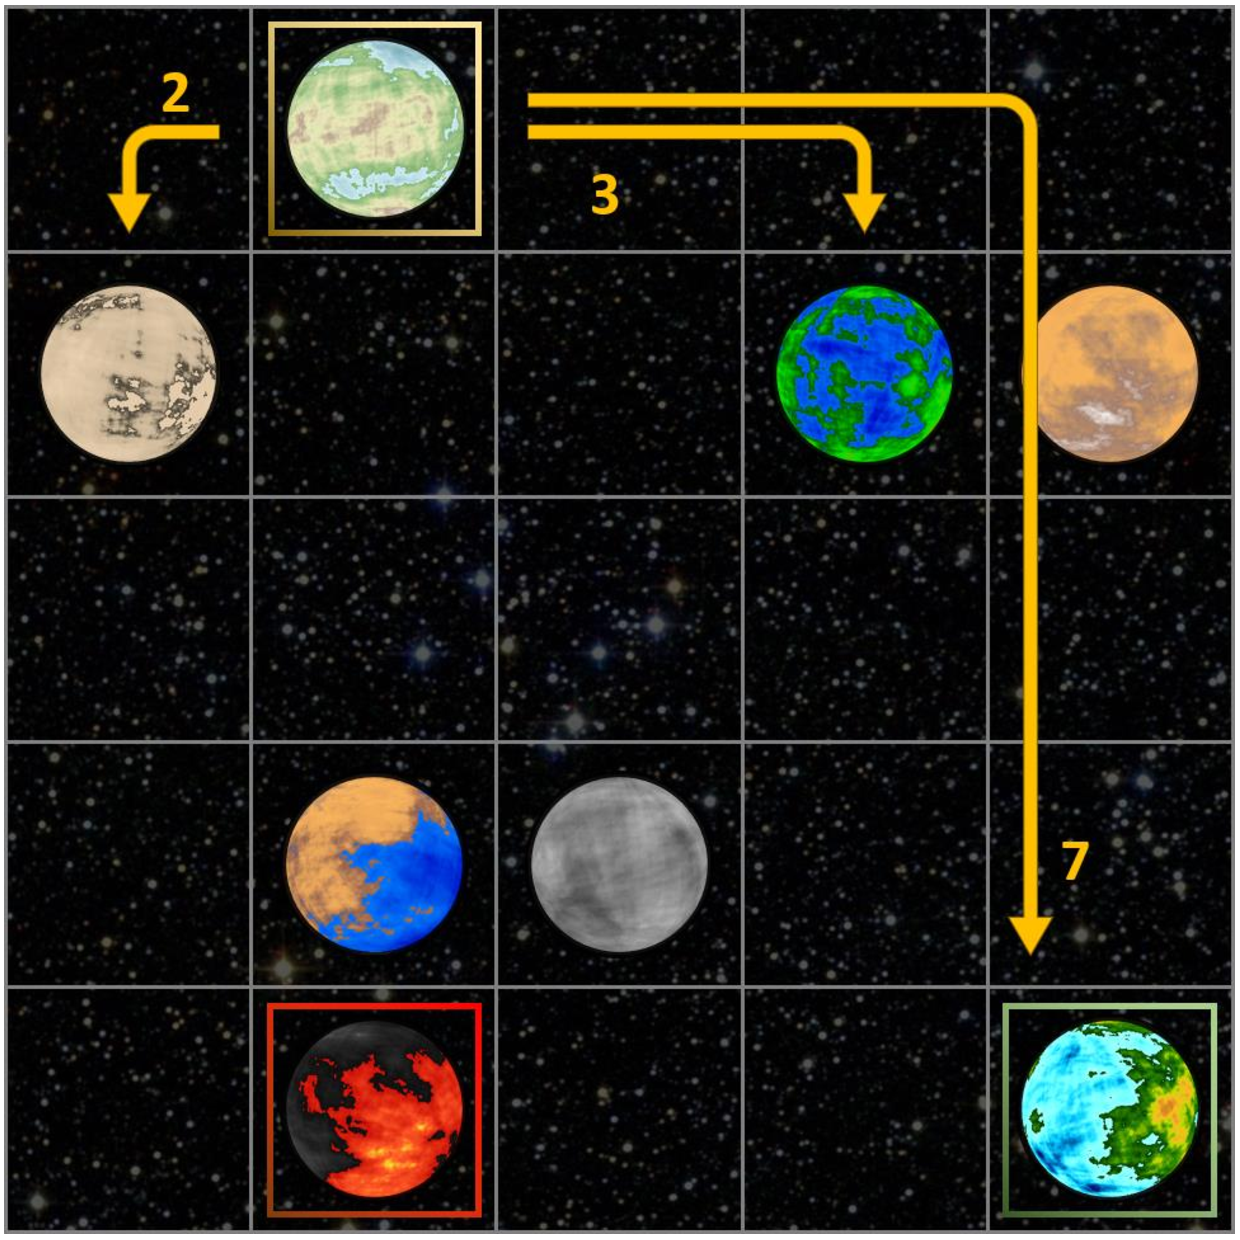
\includegraphics[width=.66\linewidth,keepaspectratio=true]{contents/images/ReachForTheStars}
		\caption{Sample game}
		\label{fig:ReachForTheStars}
	}
\end{figure}
Second, the German mobile app
\textit{Quizduell} (\citet{Quizduell.2021}) can be seen as an example for simple question-answer-games.
Last, \textit{Pen- \& Paper} role-play games and strategy games which allow more than 1 second response time e.g. through separated turns such as \textit{play-by-email} video
games (\citet{Wikipedia.2021b}) are beneficial. \\
Next, a hypothetical game is introduced, \textit{Reach for the Stars} (\hyperref[def:RftS]{RftS}) (see figure \ref{fig:ReachForTheStars}), to become less generic and abstract in the subsequent chapters.
\label{def:RftS}
After a short introduction, significant game mechanics are extracted and described theoretically.
\hyperref[def:RftS]{RftS} is a 2D, turn-based multiplayer game, where players try to colonize all planets in a sample galaxy - alike the game \textit{Risk} (\citet{Hasbro.2021}).
At the beginning, each player starts with only one planet.
Each planet has both, a fixed and a variable amount of production of space ships.
For the variable amount, \textit{randomization} is needed.
From a controlled planet, fleets can be sent to colonize/conquer other planets.
Fleets need fixed game-rounds, based on grid distance to reach planets (Figure \ref{fig:ReachForTheStars}, arrows with grid distance).
Fleet movements are not visible for the other players.
Hence the game lives from the nature of \textit{hidden transactions} and consequently originating \textit{fog of war} (\citet{By.2011}; \citet{Hagelback.2008}; \citet{Setear.1989}).
Fleets can be called back to the origin planet (once), but can not change the direction otherwise (\textit{Follow-Up hidden transactions}).
For the sake of reduced complexity colonization as well as battles are computed by linear algorithms and here not further of importance.
Last, there are two piles for each player to \textit{draw cards} from.
Both decks offer equal cards, but one is a \textit{shared deck} for all players and the other is a \textit{private deck}.
The information given on the cards is not important. \\
From this \hyperref[def:RftS]{RftS}-scenario, we can extract the need for \textit{randomization}, \textit{hidden transactions} including \textit{Follow-Up hidden transactions}, \textit{fog of war} as well as mechanics for \textit{private} and \textit{shared decks} of cards.
In this regard, time constraints on local machines
(e.g. game: M.U.L.E. from 1983, \citet{Wikipedia.2021d})
, as they are not seen to be confirmable, are out of scope.
Last, as storage space on low end devices endagers gamers to keep the game,
possible considerations to reduce storage space shall be taken into account.
For these transactions and movements \hyperref[sec:SmartContract]{SCs} have to be established which can be used in a \hyperref[chap:BCT]{BCT} context. \\

\pagebreak

\FloatBarrier

\section{Game specific smart contracts}
\label{sec:GSSCs}

Although there are innumerable designs of \gls{SC}s, games offer some common patterns.
Some of these patterns like \textit{hidden transactions}, \textit{fog of war}, \textit{pile of cards} or \textit{randomization} were just mentioned and are explained together with \textit{reveal claims triggers} and \textit{disputes} subsequently:



\subsection{Hidden transactions \& Randomization}
\label{sec:HiddenTransactionsPlusRandomization}
If a game incorporates transactions which shall not be visible to other players immediately, a suitable \gls{SC} is needed. \label{lbl:HiddenTransactions}
The \textit{receiving players} have a justifiable desire to obtain a proof for the \textit{publishing player's} interaction.
Still the \textit{publishing player} wants to sustain the information, contained in the transactions, unpublished as long as possible/needed.
Hence there is a need for the information to be published 'veiled', which becomes 'unveiled' later on.
There are two approaches for this course of action, which from now on will be called \textit{offset revealing}. \\
\textbf{First}, the \textit{publishing player} uses \textbf{encryption} to veil the information and pushes it into the \gls{BC} network.
By the time the needed information has to be revealed, the password of the encryption is published.
As all nodes do not trust each other, they recalculate the transaction with the newly published key.
\textbf{Second}, only the hash of the transaction data \textbf{game hash} could be published \cite[94]{Kraft.2016}.
Both solutions offer benefits and downsides. \label{def:GameHash} \\
On the one hand, a \textit{game hash} is lightweight ($\sim0.032$ KB)\footnote{\hspace{0.1cm}The SHA256-algorithm generates fixed size 256-bit (32-byte) hashes \cite[7]{Rachmawati.2017}.}
and abstracts from the actual storage size of the transaction.
On the other hand, encryption allows to pass the decryption key to single elected players instead of the whole network.
If this measure is needed, \textit{game hashes} might be the inferior solution.
Hence, decryption to a part of the network becomes relatively easy/cheap in the case of encryption.
Still, encrypted data might offer implications on the content (e.g. transaction size) or the game requires data to be written unencrypted to the \gls{BC} later on.
Without using storage restoring procedures (see chapter: \hyperref[sec:DataAllocationImprovements]{Data allocation improvements}),
encryption might lead to unnecessary allocated storage.
Additionally, if there are only a few movement options, which can be iterated using 'brute force',
\textit{salt data} \cite[597]{Morris.1979} should be considered.
\begin{figure}
	\centering{
		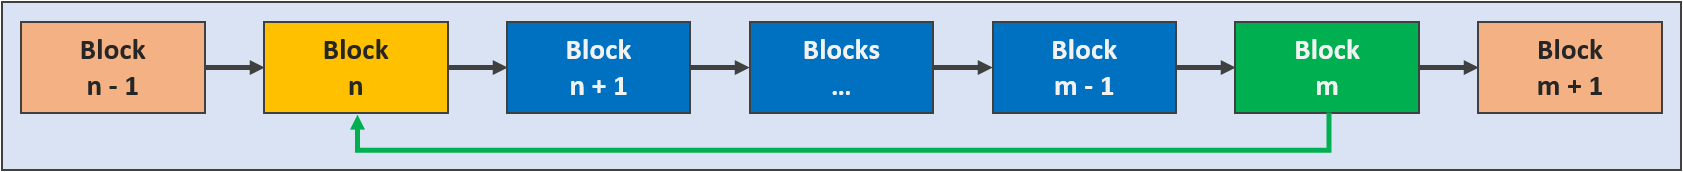
\includegraphics[width=.95\linewidth,keepaspectratio=true]{contents/images/OffsetRevealingSingle}
		\caption{Offset revealing of a single block (As described by \citet{Kraft.2016})}
		\label{fig:OffsetRevealingSingle}
	}
\end{figure}
\noindent However, the \gls{BC} itself would look like figure \ref{fig:OffsetRevealingSingle}
which aligns the blocks according to their publication time from \textit{old} (left) to \textit{new} (right).
In figure \ref{fig:OffsetRevealingSingle} there are blocks 'before \textbf{m-1}', 'after \textbf{p+1}' and 'in between the revelation \textbf{m+1} to \textbf{p-1}'.
Block \textbf{m} equals either the encrypted or hashed data,
whilst block \textbf{p} equals the encryption key or the data described by the hash.
Block \textbf{p} reveals the information contained in block \textbf{m} to the network. \\
This procedure can be used for semi-simultaneous turns as well \cite[94]{Kraft.2016}.
Here 'simultaneous' does only refer to the game play - depending on the \hyperref[sec:ConsensusMechanisms]{CM},
the network can both be \textit{sequential} (e.g.: \gls{PoP}) or \textit{semi-parallel} (e.g.: \gls{PoW}). \\
In \citet[22]{Yuen.2019}'s paper, which introduces \gls{PoP},
a procedure for \textit{simultaneous hidden turns} is given alike figure \ref{fig:OffsetRevealingGameHash}.
\begin{figure}
	\centering{
		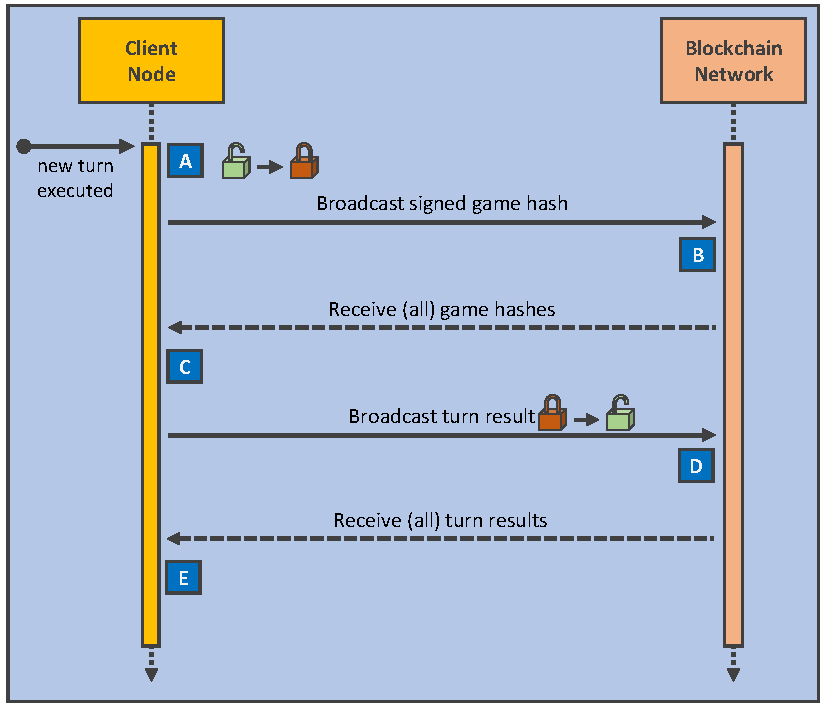
\includegraphics[width=.72\linewidth,keepaspectratio=true]{contents/images/OffsetRevealingGameHash}
		\caption{Offset revealing with game hash (From \citet{Yuen.2019})}
		\label{fig:OffsetRevealingGameHash}
	}
\end{figure}
\noindent In this case, multiple players have to publish any kind of information \textit{simultaneously}.
The recent transaction's \textit{game hash} will be encrypted (Figure \ref{fig:OffsetRevealingGameHash}, A) and sent (Figure \ref{fig:OffsetRevealingGameHash}, B).
Comprehensibly, none of the players wants to reveal the information before the other has not published his information in the \gls{BC}.
Hence it is waited until all involved nodes have published their \textit{game hash} (Figure \ref{fig:OffsetRevealingGameHash}, C).
As soon as all information is gathered, the information is released (Figure \ref{fig:OffsetRevealingGameHash}, D).
Finally, all players could make their moves simultaneously and check the other peer's results (Figure \ref{fig:OffsetRevealingGameHash}, E). \\
Consequently, synchronous and asynchronous as well as solo, paired and grouped hidden transactions can be served with this type of \gls{SC}s. \\

\noindent \textbf{Hidden follow-up movements} \\
Likewise to figure \ref{fig:OffsetRevealingSingle}, in a game a following transaction might occur, which implies the existence of the base transaction (Figure \ref{fig:OffsetRevealingFollowUp}). \label{lbl:FollowUpMoves}
This type of transactions for \gls{BCT} has not yet been described in the literature. \\
To stay within the context of \hyperref[def:RftS]{RftS} a fleet, sent to any planet, is called back before its arrival at the intended location.
This movement is only allowed given the side constraint that it has to return to its planet of departure.
Additionally, such a maneuver can only be performed once within a fleet-sending procedure. \\
As long as the implementation dependent \textit{maximum time to hide information} is not exceeded, \textit{hidden follow-up movements} are possible.
On a more abstract level, in figure \ref{fig:OffsetRevealingFollowUp},
\textbf{m} is the base transaction enhanced by the follow-up transaction \textbf{n}.
Both \textbf{m} and \textbf{n} are revealed by block \textbf{p}.
In figure \ref{fig:OffsetRevealingFollowUp} the hidden follow-up movement is consequently finished before block \textbf{p+1} is published.
\begin{figure}
	\centering{
		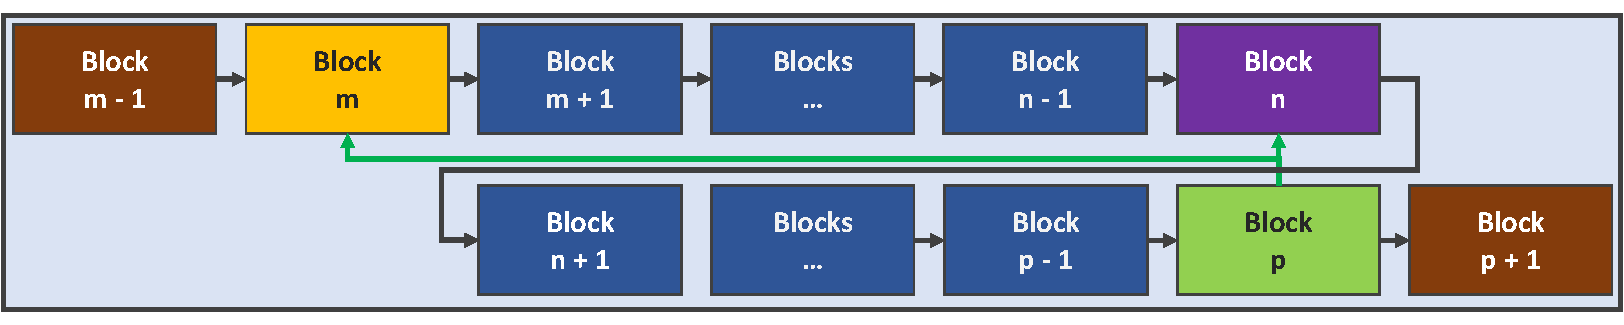
\includegraphics[width=.95\linewidth,keepaspectratio=true]{contents/images/OffsetRevealingFollowUp}
		\caption{Offset revealing with follow up}
		\label{fig:OffsetRevealingFollowUp}
	}
\end{figure}
\noindent If not intentionally, in a poor design of upper level software, the node may be enforced to publish block \textbf{m}
before the fleet has returned to the planet it has originated from.
Hence block \textbf{m} needs to be published by e.g. any \textit{timeout rule}.
The timeout implies (assumption) that the fleet would have had to reach the destination planet already.
Consequently block \textbf{m} represents an inconsistency.
Therefore, at least a statement has to be published that the
fleet's callback has occurred somewhere in between.
Now: 
\begin{enumerate}
	\item The range of rounds for the revisit of the fleet at its origin country to occur becomes limited.
	\item If there is only one block left which could represent the callback, the hidden follow-up movement is revealed by implication.
	The number of rounds between sending and calling back offers all players to calculate the round for the fleet to return.
	\item If the \textit{timeout rule} is set very low, block \textbf{n} has to be published as well before the fleet has finally returned.
\end{enumerate}
As the implications of \textit{hidden follow-up movements} are known, further details remain implementation dependent. \\

\noindent \textbf{Randomization} \\
Randomization in a distributed network needs \textit{hidden transactions} as well as \textit{trigger events} (section \hyperref[sec:RcTeDisputes]{Reveal claims, trigger events \& Disputes}). \label{lbl:Randomization}
To compute (pseudo) random values a common procedure is to take a \textit{random number generator} and give it some sort of \textit{seed}.
Mostly something alike the \textit{system clock time} or requested \textit{random mouse movement} etc. is used.
Nevertheless, if one node \textbf{P} needs a random number, other players might not comply with \textbf{P}'s local generated number - a lack of trust into \textbf{P}'s seed exists.
\citet{Chatterjee.2019} address this phenomenon in detail and describes four approaches to solve the problem.
Herein \citet{Chatterjee.2019} discourage from three of these approaches:
\begin{enumerate}
	\item The last block's hash can be seen as a random value,
	therefore it can generally be used as a seed \cite[403]{Chatterjee.2019}.
	Still, using a value from "[...] the current block as a seed [...]" \cite[403]{Chatterjee.2019} is seen not desired
	as the previous block may be tempered by a party which has interest into a 'fitting' random value \cite[406]{Chatterjee.2019}.
	\citet{Harkanson.2020}'s approach targeting 'Texas Hold’em Poker' can be put in this category.
	
	\item Alternatively an external provider could be used who acts as an oracle for the network \cite[403]{Chatterjee.2019}.
	This solution is out of scope as it requires a trusted external source.

	\item \citet{Chatterjee.2019}'s own algorithm may be used.
	In this case a \gls{BC} environment has to be used 
	which enforces to pay fees \cite[403]{Chatterjee.2019}.
	This solution is encouraged by \citet[403]{Chatterjee.2019}, but the fees in
	form of cryptocurrency tokens are seen as a flaw is this document's context.

	\item Last, the "anyone can submit randomly-generated numbers" \cite[403]{Chatterjee.2019} approach.
	Although \citet[406]{Chatterjee.2019} discourage from conducting this approach, it is given in more detail
	as one of \citet[406]{Chatterjee.2019}'s grounding assumptions can be changed. \\
	But first, the process:
	For the sake of simplicity a simultaneous hidden turn is assumed after a trigger call from \textbf{P} (Figure \ref{fig:OffsetRevealingGameHash}).
	Node \textbf{P} offers a \textit{game hash} which represents
	a certain number for the seed (Figure \ref{fig:OffsetRevealingGameHash} \& table \ref{tbl:RandomizationValues}: \textbf{B}).
	Subsequent \textbf{P} awaits other nodes to add their desired values as well (Figure \ref{fig:OffsetRevealingGameHash} \& table \ref{tbl:RandomizationValues}: \textbf{C}). \\
	Depending on the implementation, \textbf{P} waits until at least one answer arrives or 'a certain time is passed' \cite[406
	]{Chatterjee.2019}.
	On the one hand, the '\textit{at least one answer}'-solution may stall the network - if no answer is given.
	On the other hand, the '\textit{time based}'-solution may lead to attempts to choose a time slot
	which gives no answer and node \textbf{P} picks the most desired seed alone,
	which breaks the intention of randomization. \\
	Once the values are given or the time slot has exceeded, the values are revealed
	(Figure \ref{fig:OffsetRevealingGameHash} \& table \ref{tbl:RandomizationValues}: \textbf{D}) \cite[406]{Chatterjee.2019}.
	After all given values are revealed (Table \ref{tbl:RandomizationValues}: X, Y \& Z in \textbf{D}) or time has exceeded
	(Table \ref{tbl:RandomizationValues}: $\alpha$ in \textbf{D}), \textbf{P} calculates the seed
	out of the given values (Table \ref{tbl:RandomizationValues}: \textbf{E}).
	For the sake of tangibility a simple \textit{sum} is used here.
	Last, \textbf{P} receives a random number out of a predefined \textit{static random generator} (Here: Random of ($1,522$)).
	During the randomization procedure, once a (hidden) seed is given, no adjustment is possible.
	Additionally, none of the participating nodes (\textbf{P, Q, R, S \& T}) can adjust their value to that
	of the others as the one-way hash functions prevent altering in between \cite[406]{Chatterjee.2019}.
	\begin{table}[!b]
		\centering
		\begin{tabularx}{0.83\textwidth}{ c | c | c | c | c }
			\textbf{Node\textbackslash State} & \textbf{Start (B)} & \textbf{Answers (C)} & \textbf{Reveal (D)} & \textbf{Calculation (E)} \\ \hline
			\textbf{P} & X & $-$ & $X = 412$ & $-$ \\ \hline
			\textbf{Q} & $-$ & Y & $Y = 369$ & $-$ \\ \hline
			\textbf{R} & $-$ & $-$ & $-$ & $-$ \\ \hline
			\textbf{S} & $-$ & $\alpha$ & $\alpha = ???$ & $-$ \\ \hline
			\textbf{T} & $-$ & Z & $Z = 741$ & $-$ \\ \hline
			\textit{Seed} & $-$ & $-$ & $-$ & $\sum_{\substack{X,Y,Z}} = 1,522$ \\ \hline
		\end{tabularx}
		\caption{Sample given randomization values}
		\label{tbl:RandomizationValues}
	\end{table}
	Finally, the randomization's process outcome is dependent on every involved node and
	'\textit{non participating}'-nodes cannot veto (afterwards) because they are guilty in the case of '\textit{not participating}'.
	
	
	\citet[406]{Chatterjee.2019} sees a flaw in this approach as the time slot of revealing
	each seed (Table \ref{tbl:RandomizationValues}: \textbf{D}) offers the possibility to alter the sum.
	If node \textbf{S} had calculated the sum and came to the conclusion that revealing $\alpha$ would lead to a less desirable random value, \textbf{S} would gain an advantage from revealing late.
	This results in two possible shots for each node \citet[406]{Chatterjee.2019} except the demanding node (this one has to be revealed anyways) and a race to become the last emitting node.
	This scenario only beholds true if each node reveals directly to the whole network.
	On the contrary any other node (e.g.: \textbf{Z}) can add a transaction containing its encrypted value.
	The transaction containing \textbf{Z}'s encrypted value is now part of the \gls{BC}.
	Assuming that there is one node \textbf{P} who asked for a random number,
	\textbf{Z} sends the key only to \textbf{P}.
	Only \textbf{P} can therefore obtain \textbf{Z}'s value during the revelation time slot.
	After the revelation time slot is over, either \textbf{P} or \textbf{Z} reveal
	the key which offers the seed to the whole network.
	Of course this additional step slows down the answer. \\	
	Against \citet[406]{Chatterjee.2019}'s claim that the process "[...] provides no incentives to the participants to submit random numbers [...]", incentives are seen here in the upper level game itself.
	Therefore same results from constantly given static values is inapplicable here as well \cite[406]{Chatterjee.2019}.
\end{enumerate}
It has to be kept in mind that random number generators need to fit the purpose and are likewise encryption, a key attack vector.
Although the thoughts are backed by \citet{Chatterjee.2019}'s paper, the solution is considered intuitive
and supposed for short time frames to cover recalculation risks etc.
It is not error prone by definition.
Although further details regarding random number generators are not in the scope of this document.
	
\subsection{Piles of Cards}
\label{sec:PileOfCards}
Dealing with cards, such as on a player's hand, in a pile or currently being drawn
can be difficult regarding security in a \hyperref[chap:BCT]{BCT} context. \label{lbl:CardDraw}
Any type of the subsequent \textit{card draw scenarios in \gls{BCT}} 
cannot be found in the literature at the present time. \\
The easiest part is distinguishing between a secret hand, just visible to the owner and an open hand, visible to all players.
Moreover decks/piles need to be shuffled or drawing has to be grounded on randomization.
Consequently, drawing cards from decks introduces specific obstacles.
The different cases are shown in table \ref{tbl:Card draw scenarios}. \\
On the one hand it is distinguished here between \textbf{private} and \textbf{public} piles in the means of accessibility.
On the other hand draws differ in regards of \textbf{open}, \textbf{private} and \textbf{hidden}
transactions in the means of visibility/openness to other players. \\
In \textbf{open} transactions a card is shown directly to all players - no restrictions in regards of accessibility exists.
In contrast, \textbf{hidden} transactions are only known to the acting player.
Other players have no indication that a card has been drawn at all - still the acting player receives a card with the attached information.
In between \textit{open} and \textit{hidden} there are \textbf{private} transactions,
which show other players that a card has been taken from the pile, but the card's information is only revealed to the drawing player.



\subsubsection{General draws from piles}
\label{sec:GDfP}
The different types of draws work as follows:
\begin{enumerate}	
	\item A \textbf{private pile} with \textbf{public draw} is supposed to be the least obstacle.
	The cards in the pile are supposed to be known by everyone and only the card to be drawn has to be determined.
	A random number helps to choose the card to be drawn (by index).
	Finally, the card is shown to all players.
	
	\item More complicated is a \textbf{private pile} with \textbf{private draw}.
	Still it is manageable as the drawn card can be proven by \textit{offset revelation}.
	Here the effective pile is only known to the drawing player in regards of order (shuffled cards).
	Again, a random number helps to choose the card to be drawn.
	The draw has to be execute as a hidden transaction for later verification.
	Still the validity of every played card may only be verifiable at the end of the game.
	The latter is e.g. depending on the fact whether the cards in the pile are generally known to other players or not.
	
	\item A \textbf{private pile} with \textbf{hidden draws} needs another mechanism.
	Already a call for randomization, the process to receive random values, implies to draw a card.
	Still, without this call a draw is not supposed to be possible.
	Contrariwise the absence of a \textit{call for randomization} implies that no card can be drawn.
	Therefore faked draw transactions are the consequence.
	But even faked draw transactions have to be documented on the \hyperref[sec:BCI]{BC} to fulfill the promised transparency and trust.
	This aspect will be covered in more detail in the section \hyperref[sec:DataAllocationImprovements]{Data allocation improvements}.
	
	\begin{table}
		\centering
		\begin{tabularx}{0.525\textwidth}{ l | c | c | c }
			\textbf{Pile\textbackslash Draw} & \textbf{Open} & \textbf{Private} & \textbf{Hidden} \\ \hline
			\textbf{Private} & \textbf{1.} & \textbf{2.} & \textbf{3.} \\ \hline
			\textbf{Public} & \textbf{4.} & \textbf{5.} & \textbf{6.} \\
		\end{tabularx}
		\caption{Extended Blockchain Network Types}
		\label{tbl:Card draw scenarios}
	\end{table}
	
	\item A \textbf{public pile} with \textbf{public draw} is supposed to be as easy as a \textit{private pile} with \textit{public draw} (\textit{1.}).
	The only difference is that all players can access the pile to draw from it - the pile is not explicitly reserved for one specific player.
			
	\item A \textbf{public pile} with \textbf{private draw} is supposed to be the most complex situation
	as it requires the highest level of collaboration. \\
	Therefore, it is moved to the following section (\hyperref[sec:PPwPd]{Public pile with private draw}).
	
	\item Last, a \textbf{public pile} with \textbf{hidden draw} offers a special mutually exclusive case.
	As this type prevents to inform other nodes that a card was drawn,
	not even the drawn index from a multiple times shuffled and encrypted pile is allowed to be published.
	Consequently, a node in a subsequent turn may draw an already taken card from the pile.
	Hence a race condition \cite[75]{NetzerR.H.B..1992} in the form of \citet{Nakamoto.2009}'s \textbf{double spending problem} occurs.
	To the current knowledge, this problem connot be solved without external help,
	such as \hyperref[sec:HelperNodes]{Helper Nodes}. 
	These are discussed in further detail in the section
	\hyperref[sec:FurtherCharacteristics]{Further Characteristics} of the \hyperref[chap:PoT]{Proof-Of-Turn} approach.
\end{enumerate}



\subsubsection{Public pile with private draw}
\label{sec:PPwPd}
The key issue of this type is that only the drawing player is allowed to receive the card's information.
Nevertheless, the other players are not allowed to draw the same card from the pile thereafter.
Hence, they need to know which card's placeholder (e.g. index) was taken.
Naturally, the index is not allowed to reveal the cards information/identity.
A mechanism has to be implemented, which hides the cards information, but prevents overlapping transactions (double spending) from the pile.
To untangle the challenge, the single card's information and the card's destination in the pile need to be separated to provide a suitable placeholder mechanism.
This can be done by shuffling and encrypting the cards.
Still, the 'shuffling and encrypting'-party has full knowledge about both the previous as well as the subsequent state of the pile.
Therefore several parties have to be involved. \\
During the process at least two rounds of 'shuffling and encryption' are needed and at least three parties have to participate.
Basically, with every additional party, another round of 'shuffling and encryption' has to be conducted.
The first round of encryption has to be executed using asymmetric encryption.
The asymmetric encryption has to be split on two (distinct) parties, one encrypting and another offering the decryption keys.
Last, a third party is needed to prevent data exposure.
The process is given in more details in Figure (\ref{fig:NodesShufflingCards}) and the steps and their possible pitfalls are described hereafter. \\
\begin{figure}[!b]
	\centering{
		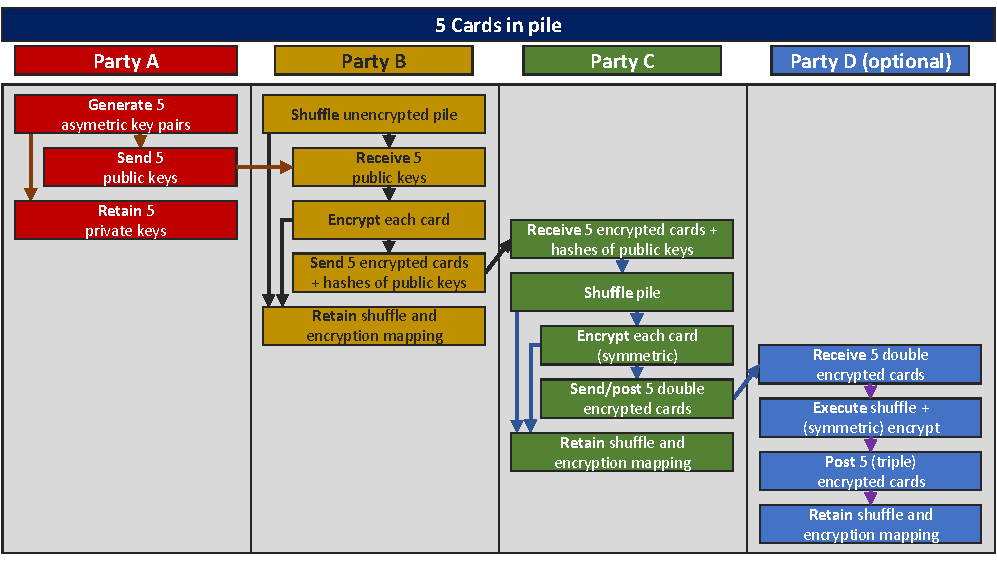
\includegraphics[width=.95\linewidth,keepaspectratio=true]{contents/images/ShuffleCardsNodes}
		\caption{Parties shuffling cards}
		\label{fig:NodesShufflingCards}
	}%
\end{figure}
\noindent First \textbf{Party A} creates asymmetric encryption key pairs for each card.
\textit{Party A} is not allowed to encrypt the cards.
If \textit{Party A} would encrypt the cards, it would become the single gatekeeper and knew every drawn card.
Hence \textbf{Party B} shuffles the unencrypted pile and then encrypts each card using the (public) keys received from \textit{Party A}.
Without \textit{Party B}'s shuffling the encryption would be useless as the \textit{default pile} is known.
The resulting pile, consisting of encrypted cards complemented with their key's hash, is therefore (only) given to \textit{Party C}.
At this moment \textit{Party A} is not allowed to be involved, as it could decrypt all cards to receive the pile's change of order.
To prevent \textit{Party A} from decrypting, \textbf{Party C} shuffles to diminish \textit{Party B's} knowledge (Indexes) and encrypts each card again to prohibit \textit{Party A's} access.
Now none of the parties is capable to access information from the pile without consultation of all other parties. \\
More precisely, after the process: \textbf{Party A} does not have access to the pile unless \textit{Party C}
grants permission and hands over a card which is only encrypted with one of \textit{Party A}'s public keys.
\textbf{Party B} knows the first pile's change of order (from origin), but does neither know \textit{Party C's} shuffle nor \textit{Party A's} private keys.
Last, \textbf{Party C} neither has \textit{Party A's} private keys, nor \textit{Party B's} change of order to the source pile.
Consequently, the resulting \textbf{twice} \textit{shuffled and encrypted} pile can then be written to the \gls{BC}.
During the game the pile's cards are drawn numbers (Indexes).
Each party knows which card has been drawn from \textit{Party C}'s published pile as the drawn indexes are known.
This solves the 'double spending' challenge. \\
To the knowledge of the author, there is no possibility to decrease the number of parties below three.
Nevertheless, an infinite number of parties can be added between \textit{Party C} and the publication of the pile, represented in figure \ref{fig:NodesShufflingCards} by \textbf{Party D}.
Each added party reshuffles the pile and encrypts it with its own keys, just as \textit{Party D}.
Except the mandatory asymmetric encryption used by \textit{Party A} and \textit{Party B}, all other encryption is free to use either a symmetric or asymmetric encryption procedure.
Naturally, with each additional party, the reconstruction becomes more intricate.
Generally only the shuffling is needed until \textit{Party B}'s encrypted card can be combined with \textit{Party A}'s key to retrace the final information.
But in a hostile environment, each party insists on full safety/transparency.
Hence, on each step towards decryption, the drawing party insists on proof of correctness.
Thus, for not getting tricked, the key on every stage is claimed and validated. \\
If the key does not work properly (e.g. wrong data was transmitted),
the sending party has to be blamed directly, as it might try to betray (the network).
Additionally, the party which is asked to provide the card's information claims valid input data to ensure that
particularly this card is chosen and has to be revealed (especially for Party A's private keys).
Hence, the \textit{encrypted information} from the previous party,
which equals to one of the asked party's produced cards \textit{plus} its \textit{corresponding index} have to be delivered.
Only if \textbf{both values} are supplied, representing a valid claim to receive information, data is provided. \\
In figure \ref{fig:ShuffledCardsDecryptionAtoC} the decryption processes for the \textit{parties A, B and C} are shown.
Given the case that there are more than three parties, such as another \textit{Party D} and beyond, the adapted process is shown in figure \ref{fig:ShuffledCardsDecryptionMultiple}.
\begin{figure}
	\centering{
		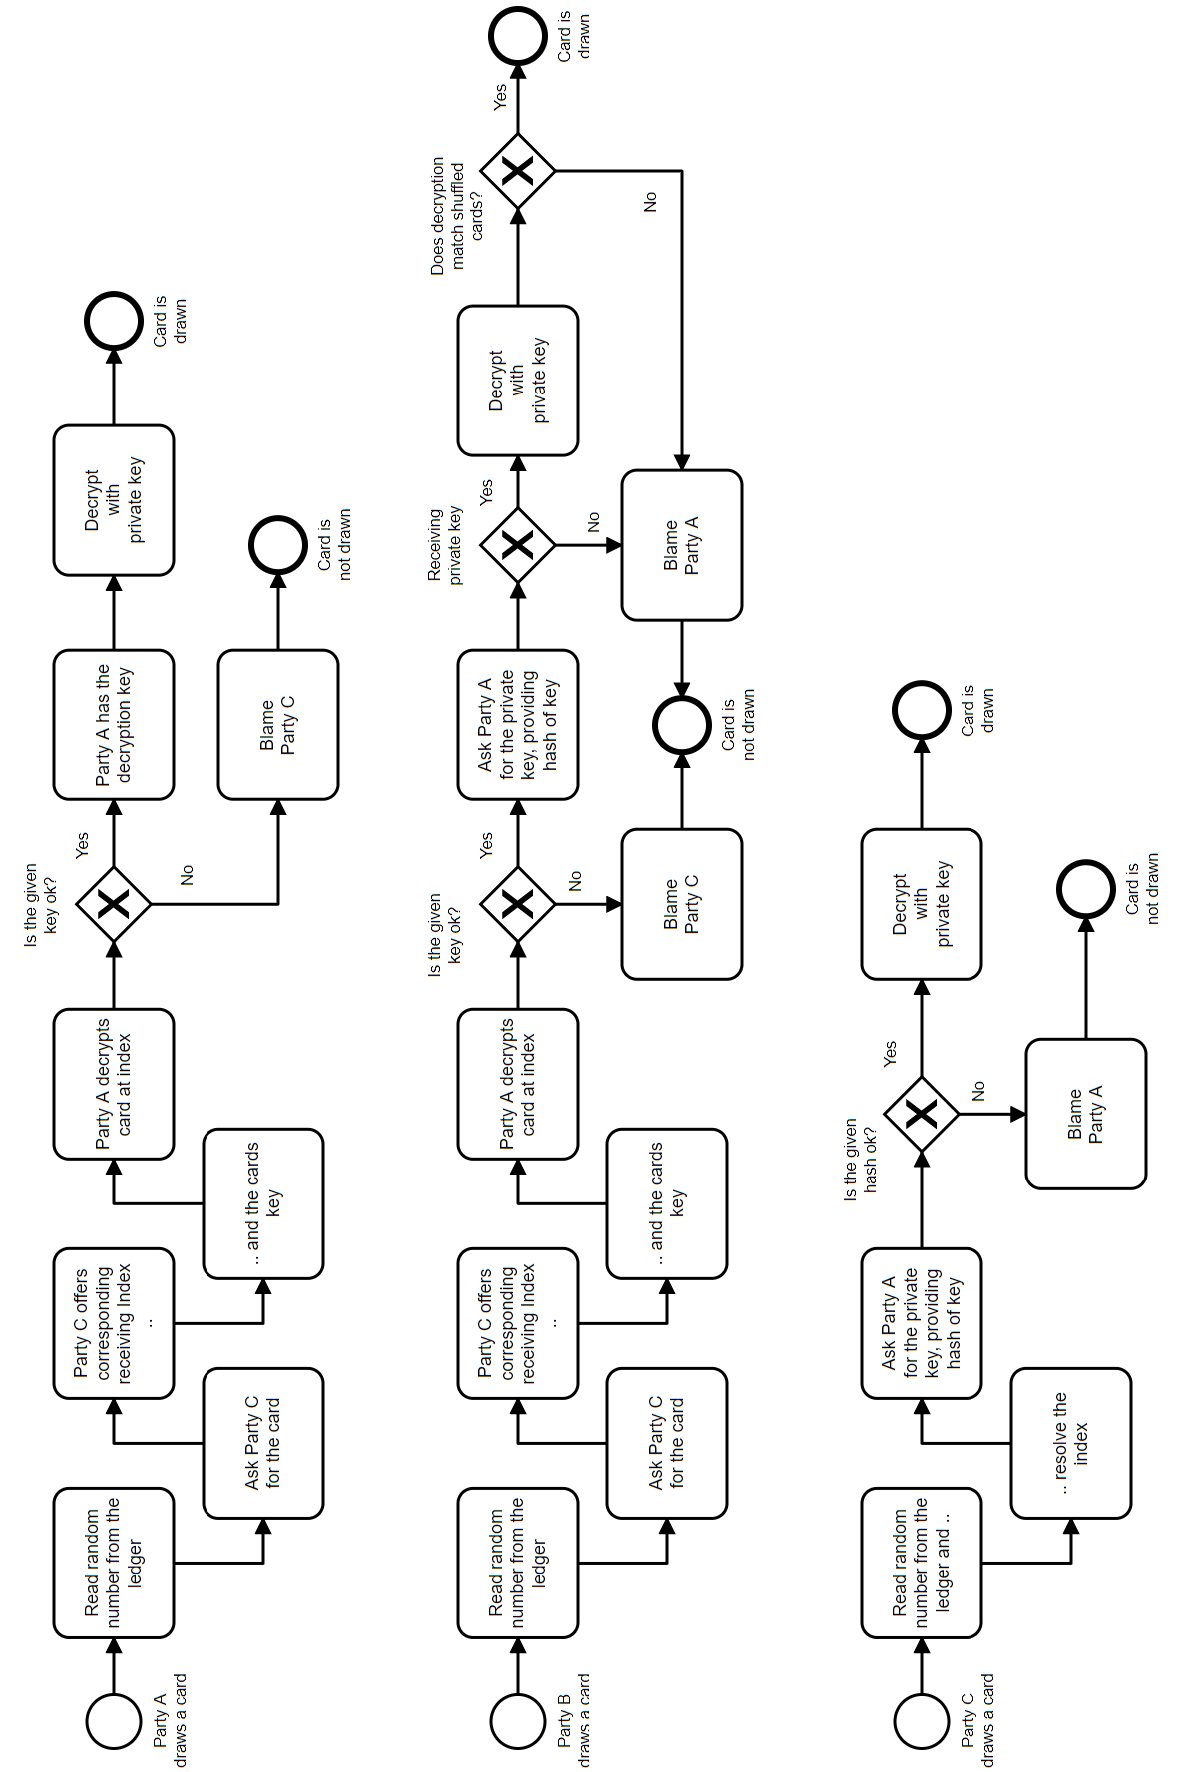
\includegraphics[width=.95\linewidth,keepaspectratio=true]{contents/images/ShuffleDecryptNodeAtoC90}
		\caption{Decryption processes (Nodes A, B and C)}
		\label{fig:ShuffledCardsDecryptionAtoC}
	}
\end{figure}
\begin{figure}
	\centering{
		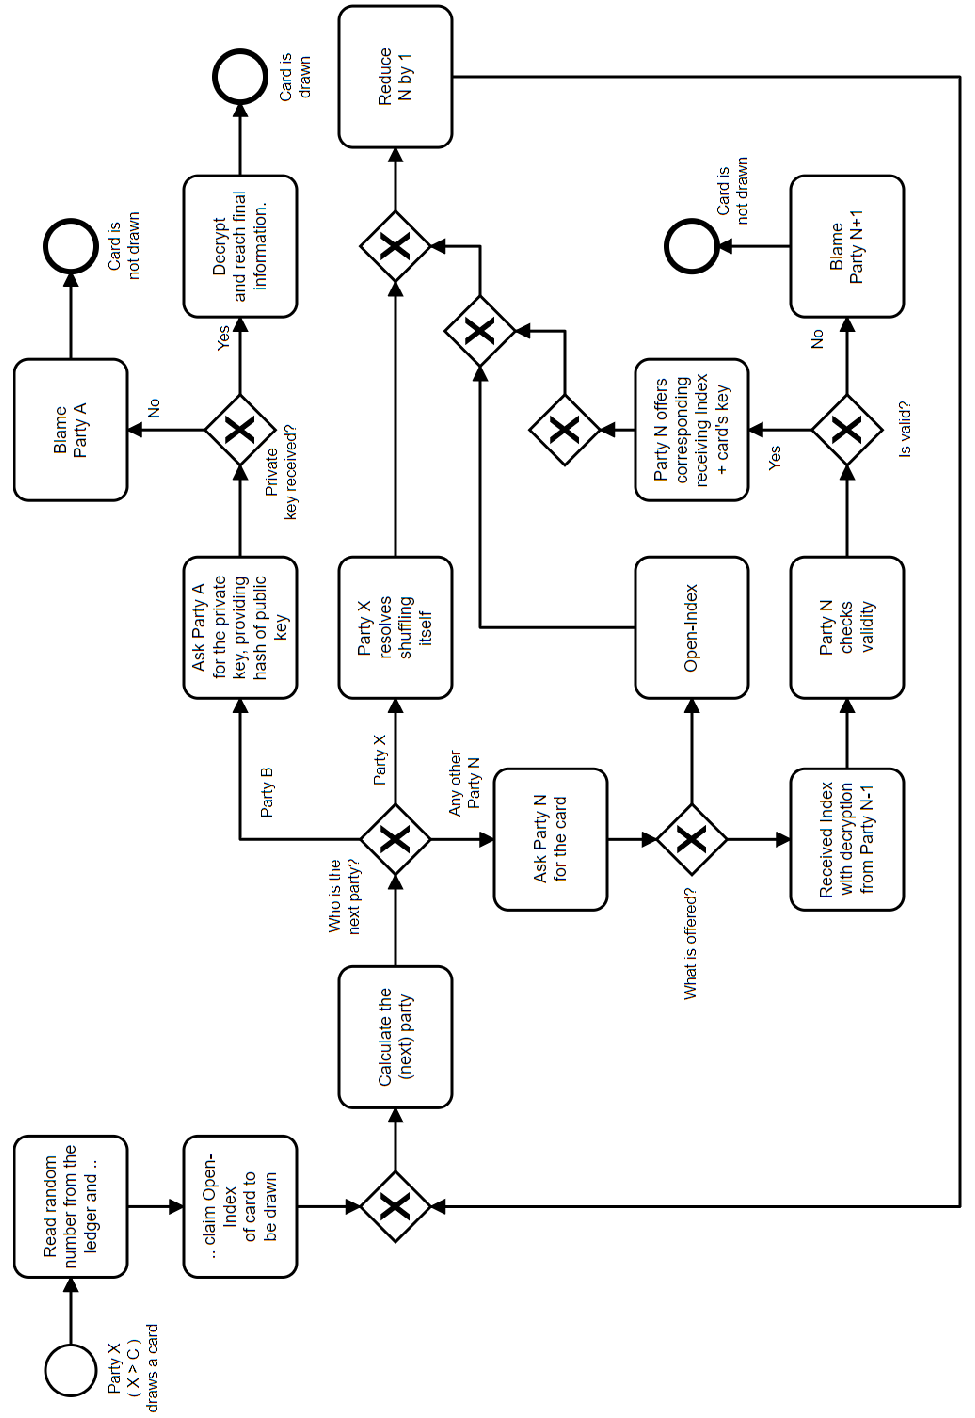
\includegraphics[width=.87\linewidth,keepaspectratio=true]{contents/images/ShuffleDecryptNodeDtoN90}
		\caption{Decryption processes using many nodes ($\geq D$)}
		\label{fig:ShuffledCardsDecryptionMultiple}
	}
\end{figure}

\noindent Note that there are pitfalls if wrong information is transmitted or a party, which has to offer specific information, is not available.
This shows a major problem of this solution and stresses why recently it was not talked about \textit{network nodes}, but rather about \textbf{parties}.
The case of unavailability of any node, for whatever reason, freezes the network.
If the network freezes as described in the \textbf{Multichain} approach, there is no possibility to recover unless the affected node reconnects to the network.
Thus a game designer has to choose between a full mistrust scenario and cooperation of nodes.
In a three players game - as mentioned before the minimum amount of players - each node has to become one of the three parties.
But if there are more nodes participating in the process, a party may consist of multiple nodes as well.
The latter decreases trust and reduces security.
Still, if multiple nodes are capable to provide needed information responsiveness of the network rises.
This is especially desirable because the decryption as well as the shuffle trace back can only be performed in one specific order.
A review of the \hyperref[sec:ByzantineFaultTolerance]{BFT} problem to ensure fraud resilience has to be conducted.
\textit{Fraud resilience} follows the graphs shown in
figure \ref{fig:ShuffleCards}\footnote{\hspace{0.1cm}Figure \ref{fig:ShuffleCards} plot's Python code is given in the \hyperref[script:BFTshufflingCards]{appendix}.}.
Assuming \textbf{full mistrust} (Figure \ref{fig:ShuffleCards}: $\delta$), starting at a minimum of three nodes, all nodes would need to turn hostile to decrypt information.
Hence, no node can trick another or the whole network.
Nevertheless, it is the most vulnerable type in regards of a \textit{frozen network} state.
\begin{figure}
	\centering{
		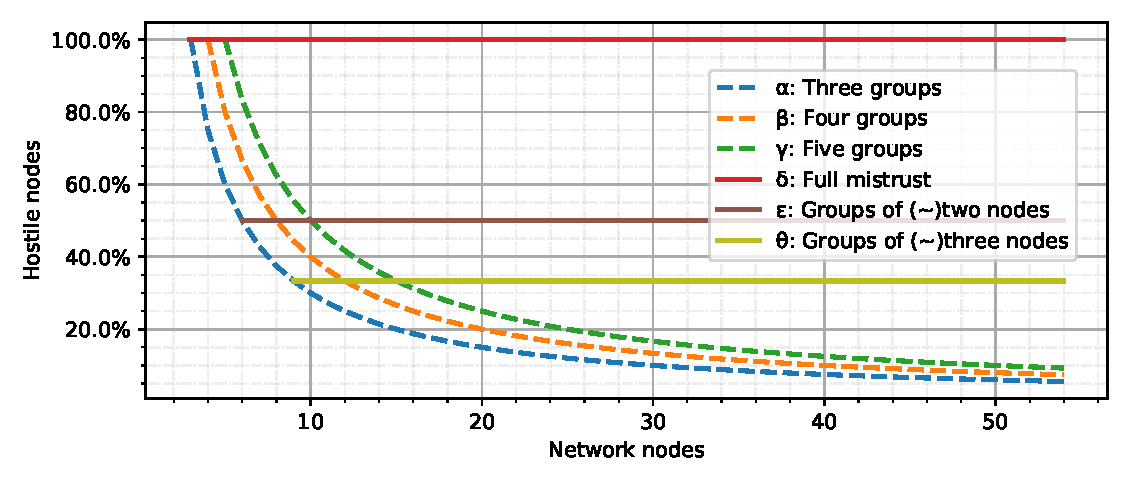
\includegraphics[width=.95\linewidth,keepaspectratio=true]{contents/images/ShuffleCardsGraph}
		\caption{BFT shuffling cards}
		\label{fig:ShuffleCards}
	}
\end{figure}
Increasing the number of nodes able to provide the information leads to the graphs $\epsilon$ and $\theta$.
Dividing all nodes into \textbf{groups of two} (Figure \ref{fig:ShuffleCards}: $\epsilon$) implies that each group needs to contain at least one hostile node to enable fraud.
Hence at least $50.0\%$ of nodes have to become hostile to break the system.
In the best case only one group with fully honest players is able to keep the system fraudless.
An even higher redundancy, dividing all nodes into \textbf{groups of three} (Figure \ref{fig:ShuffleCards}: $\theta$), leads to at least $33.3\%$ fraud resilience.
Raising redundancy even higher as of fixed \textbf{three, four or five groups}
containing many nodes (Figure \ref{fig:ShuffleCards}: $\alpha$, $\beta$ \& $\gamma$) reduces fraud resilience dramatically.
Depending on the desired resilience level, $\delta$, $\epsilon$ and $\theta$ are recommended.
Nevertheless, in particularly huge games with dropping out players a low number of groups might be superior.
Here it has to be reminded of \citet{Laneve.2019} who state that \gls{BCT} "[...] is reliant on the game’s popularity to keep it running, making it a risky choice for developers" (p. 27).
The final decision remains implementation dependent.



\FloatBarrier

\subsection{Fog of War}
\label{sec:FogOfWar}
\noindent Comparable \hyperref[sec:SmartContract]{SC}s might be needed, if a game includes
\textit{fog of war} elements, which deal with uncertainty of combat situations (\citet{Setear.1989}). \label{lbl:FogOfWar}
Again, there was no literature to be found which covered \textit{fog of war scenarios in \gls{BCT}}. \\
Four general uncertainties are assumed: '\textit{enemy's intentions}', '\textit{natural environment}',
behavior of '\textit{friendly forces}' and '\textit{underlying laws of war}' \cite[3-4]{Setear.1989}.
\begin{figure}
	\centering{
		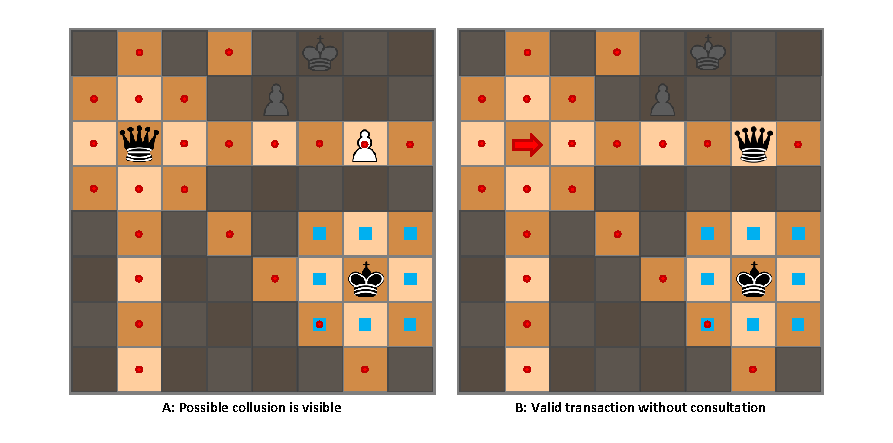
\includegraphics[width=.995\linewidth,keepaspectratio=true]{contents/images/FogOfWar_Chess_AB}
		\caption{Fog of war in chess - Open moves (1)}
		\label{fig:FogOfWar_Chess_AB}
	}
\end{figure}
The last case does not apply in this scenario as it is diminished by defined \gls{SC}s and game rules.
Nevertheless, in many (realtime) strategy games especially the first two listed uncertainties are used.
In gaming environments with a central server, which is aware of every move, this does not offer special challenges as the server can always provide all needed values.
Back in a distributed environment, a challenge similar to the previous card draw scenario occurs.
\begin{figure}
	\centering{
		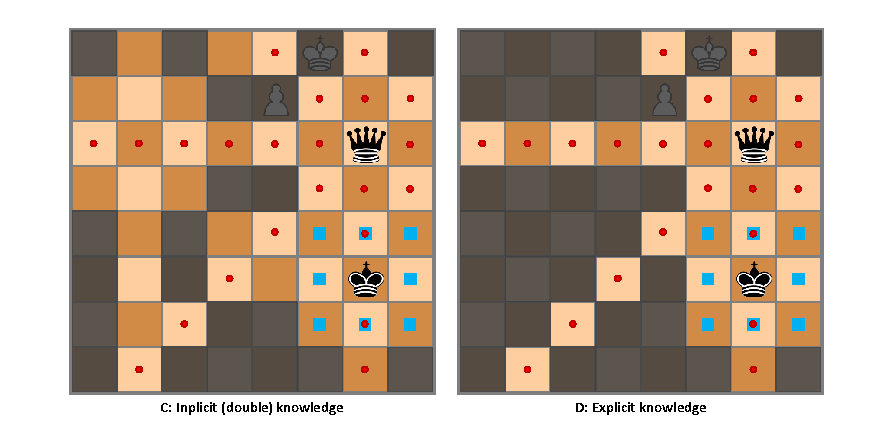
\includegraphics[width=.995\linewidth,keepaspectratio=true]{contents/images/FogOfWar_Chess_CD}
		\caption{Fog of war in chess - Open moves (2)}
		\label{fig:FogOfWar_Chess_CD}
	}
\end{figure}

\noindent \textbf{First}, the easy case:
The game is designed in a way that every possible move can only be performed on fully revealed instances (Figure \ref{fig:FogOfWar_Chess_AB}, A).
Hence, each move can be calculated by the executing node (Figure \ref{fig:FogOfWar_Chess_AB}, B).
The information for the next move will be provided during the next network round.
All other nodes provide needed data (lifting the fog) for the next round on the affected fields (Figure \ref{fig:FogOfWar_Chess_CD}, C: Squares and dots).
On those fields, which are out of the new area of visibility, fog rises again (Figure \ref{fig:FogOfWar_Chess_CD}, D).
\begin{figure}
	\centering{
		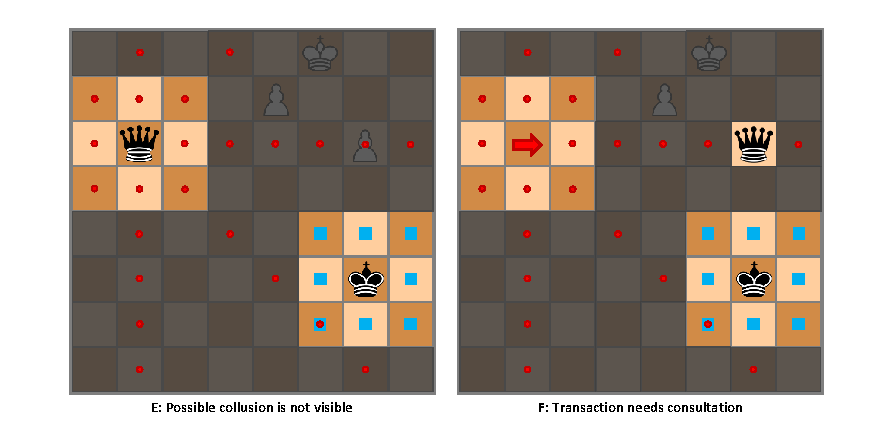
\includegraphics[width=.995\linewidth,keepaspectratio=true]{contents/images/FogOfWar_Chess_EF}
		\caption{Fog of war in chess - Fogged moves (1)}
		\label{fig:FogOfWar_Chess_EF}
	}
\end{figure}

\noindent \textbf{Second}, the tricky case:
Just as games offer the possibility to inspect another player's hand of cards, in figure \ref{fig:FogOfWar_Chess_EF} (E),
all pawns in the game can only see the (directly) adjected tiles - regardless their movement possibilities.
Hence, performing the same move as seen in figure \ref{fig:FogOfWar_Chess_AB} to figure \ref{fig:FogOfWar_Chess_CD},
the player with black pawns does not know whether the queen will hit any enemy's pawn (Figure \ref{fig:FogOfWar_Chess_EF}, E to F).
The information has to be provided by the other players (see \hyperref[sec:RcTeDisputes]{Reveal Claims} below).
Consultation is needed to complete the move.
\begin{figure}
	\centering{
		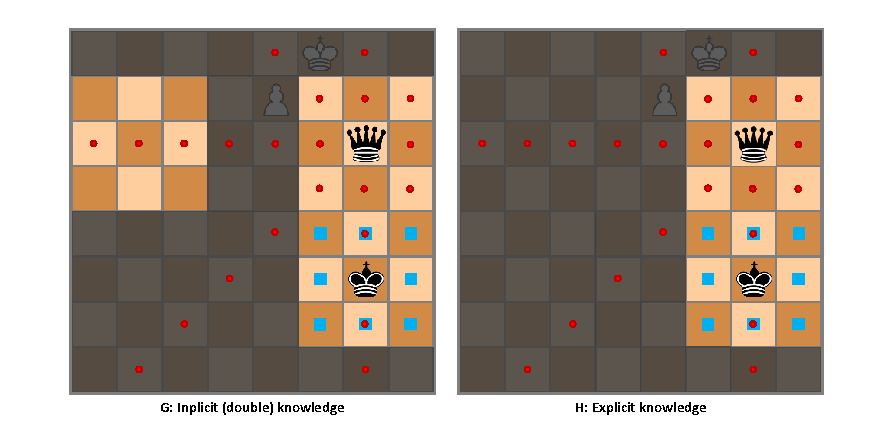
\includegraphics[width=.995\linewidth,keepaspectratio=true]{contents/images/FogOfWar_Chess_GH}
		\caption{Fog of war in chess - Fogged moves (2)}
		\label{fig:FogOfWar_Chess_GH}
	}
\end{figure}
\noindent Implications:
\begin{enumerate}
	\item All this is generally possible using \textit{hidden transactions}.
	\item Due to the rules of chess \textbf{implicit knowledge} is granted - see figure \ref{fig:FogOfWar_Chess_CD}, C as well as figure \ref{fig:FogOfWar_Chess_GH}, G -
	which is not applicable to every game.
	\item The implication, that the player in black color has to offer all other players the (new) location of his queen, makes the whole 'fog of war'-situation \textbf{pointless} - at least for chess.
\end{enumerate}
\noindent Consequently, the underlying mechanisms two (\textit{implicit knowledge}) and three (\textit{pointlessness}) need to be considered throughout during a game's development process. \\
Point two and three implicate that fog of war is generally not possible in distributed environments conducting \gls{BCT}, but that is not completely true.
Chess has many constraints, such as only one move per turn can be performed, which diminishes the reappearance of fog.
Additionally, chess offers binary type information, such as the true/false answer to the question:
'Is the black queen located on field B4?'.\\
\textbf{Third}, the case in between:
Other games may offer to hide information better, especially if information is given in a numeric type and no \textit{exact amount} has to be delivered.
Less cryptically, assume a \gls{SC} exists in \hyperref[def:RftS]{RftS}, which says: \\
\textbf{A)} After his turn a player has to publish the number of ships (\textbf{X}) stored on each of his planets. \\
\textbf{B)} The real number (\textbf{X}) does not need to be published directly - it can be included in a \hyperref[HiddenTransactions]{hidden transaction}. \\
\textbf{C)} The publicly accessible number has to be within the range of +-\textbf{X}\%. \\
\textbf{D)} The deviation has to be calculated from a \hyperref[lbl:Randomization]{randomization} process.
The value extracted from the randomization may stay hidden until it has to be revealed.\\
Concluding, setting the number of ships to 100 \textit{constantly} and \textbf{X} to 30, the published values vary between 70 and 130 ships.
This could be recalculated long term using the mean.
Still, with extending variables such as the \textit{production of ships} (influenced by \hyperref[lbl:Randomization]{randomization}) and changing amounts due to \textit{incoming/outgoing fleets} etc., this \gls{SC}, based on numeric values, fits the guidelines of \textit{fog of war} \cite[3-4]{Setear.1989}.
Finally, the real number of ships can be fogged in distributed environments like \gls{BCT}.



\subsection{Reveal claims, trigger events \& Disputes}
\label{sec:RcTeDisputes}

\textbf{Reveal claims and trigger events} - Some games offer the possibility to inspect another player's hand of cards,
lift the fog on specific values of the game or in case of \hyperref[def:RftS]{RftS} claim a planet's (real) number of stored ships.
Living in the assumption of multiple players ($\geq3$) the information has to be provided for one player (only), a subgroup of players or to all players.
In the first two cases, the information is only encrypted to the \textit{legitimately claiming} node(s).
Still, the information transfer needs to be backed by a \hyperref[sec:SmartContract]{SC}.
Moreover, within a game spontaneous transactions/triggers could exist.
These may either be 'throw in transactions' or previously placed \hyperref[sec:SmartContract]{SC} which are just waiting to be triggered.
Anyway, these transactions follow sequential order and can therefore be conducted using \gls{BCT}.
Moreover this has certain implications on the \gls{CM} and will therefore be covered in chapter \hyperref[chap:PoT]{Proof-Of-Turn}. \\
\textbf{Disputes} - Although \gls{SC}s and the chosen \gls{BCT} \gls{CM} shall prevent disputes, sometimes they are inevitable.
Hence, a general pattern to resolve disputes is given:
\textbf{First}, the dispute may be solved within the network.
This could be conducted by a vote - the majority (>$50$\%) wins.
This is probably a good solution for disputes among a little group within the whole game network, as stakes in the game may influence the vote in an unfair manner.
\textbf{Second}, if possible, hand the dispute to any upper level instance as shown by \citet[92]{Kraft.2016}.
\textbf{Third}, the case which shall be prevented if possible: Stop the game(-channel) and prevent an unjustified win for any involved party.
The possibilities a game offers regarding the three cases determine the options after a dispute:
\begin{enumerate}
	\item Waiting / freezing the game until an absent player/node is answering.
	During this time the unavailable player may be kicked by vote
	(see section \hyperref[sec:PeerFluctuation]{Peer-Fluctuation \& adaptive turn time} in chapter \hyperref[chap:PoT]{Proof-of-Turn},).
	
	\item Impose any additional upper level penalty against the node e.g. by the publisher \cite[407]{Chatterjee.2019}.
	
	\item Stop the game generally.
	This is only recommended if players can be measured by points already.	
	
	\item Conduct any kind of recover strategy, which is implementation dependent.
	This might not be possible e.g. if cards had been dealt with the previous presented shuffling mechanism,
	as both the associated reverse shuffle order and encryption keys are lost.
\end{enumerate}



\FloatBarrier

\section{Data allocation improvements}
\label{sec:DataAllocationImprovements}
In the literature \textit{data allocation improvements} could only be found before
data was written to the \gls{BC} - e.g. game hash vs. encrypted data \cite[94]{Kraft.2016} but not altering the \gls{BC} thereafter.
The general idea of removing data from a \gls{BC} after blocks became \gls{CF} harms the characteristic of \textit{immutability of data} (\citet[17-18]{Butijn.2020}; \citet[57]{Dib.2018}; \citet[21]{Sharma.2020}).
Nevertheless, to meet the demand of reduced data consumption (See section \hyperref[sec:GamingMarket]{Gaming market}),
ways to reduce data allocation whilst keeping a shared consistency need to be evaluated. \\
If there was no central server from the publisher, not only the information in a transaction can be withhold (\textit{hidden transactions}).
Already the knowledge about a transaction can be a non-desirable factor.
To make this more tangible, in the aforementioned game, \hyperref[def:RftS]{RftS}, a player makes a move, sending a fleet to another planet.
This fleet is stored as an encrypted block.
Any opponent can now assume, that a potential fleet is on its way and is consequently able to
calculate round by round whether the fleet may reach the one or the other controlled planet.
As a player has to proof his turn later on with \textit{offset revealing}, publishing the move (somehow) to the blockchain is unavoidable. \\
Nevertheless, moves can be hidden in noise data using dummy data, here referred as a \gls{BT}. \label{def:BloatTransactions}
No matter if a player takes a move or not, an additional (random) number of \gls{BT}s is added.
\gls{BT}s can be be recognized as such right after their revelation.
All \gls{BT}s need to be revealed to claim the win (even if its the second place).
The enforced revelation prevents \textbf{double spending} of a planet's ships into several fleets.
More details on \textit{double spending} in the section \hyperref[sec:AttackVectors]{Attack Vectors}. \\
Additionally, game mechanics define the number of rounds until \gls{BT}s
have to be revealed (e.g. 10 rounds after the last non-\gls{BT}s is revealed).
Consequently, the number of transactions can not be calculated from the number of published blocks during a turn.
Therefore the number of moves can be hidden using \gls{BT}s.
Nevertheless, there is a \textbf{downside of \gls{BT}s} as well, \textbf{data storage}.
In long lasting games with many moves and players, the number of \gls{BT}s will probably derive to a problem. \\
The following, storage size calculation is highly assumptive and strongly dependent on the application's use case.
Nevertheless, general traits of different approaches shall be shown.
Therefore, presumptive values are given: \\
If most \gls{BT}s consumed $\sim0.01$ MB and in contrast most \textbf{relevant transactions} $\sim0.1$ MB,
\gls{BT}s could be distinguished from \textit{relevant transactions} easily by size.
Hence, \textit{relevant transactions} as well as \gls{BT}s need to allocate a comparable amount of storage space.
This increases data allocation by the factor '\gls{BT}s per \textit{relevant transaction}'.
Alternatively, \hyperref[def:GameHash]{game hashes} could be used decreasing each transaction down to ($\sim0.032$ KB).
This is always recommendable if the average transaction's size exceeds the \textit{game hashes} fixed amount. \\
During the following equations a \gls{BT}$(l)$ is a large blob of bloat data augmenting a \textit{hidden transactions} whilst a \gls{BT}$(s)$ is only augmenting a game hash.
If encryption is used, the data allocation can be calculated with \textit{hidden transactions} ($h$), and the 'factor of \gls{BT}s per hidden transaction' ($f($\gls{BT}$(l))$).
Additionally, revelations ($r$) of the encryption key ($k$) to different nodes and the network have to be taken into account.
\begin{center}
	Encryption: \hspace{0.2cm} $h + f($\gls{BT}$(l)) + r * k$
\end{center}
On the contrary, \textit{game hashes} ($H(h)$) can be used for \textit{hidden transactions}.
\begin{center}
	Game hashes (i): \hspace{0.2cm} $H(h) + f($\gls{BT}$(s)) + r * k$
\end{center}
If a \textit{hidden transactions} (game hash) has to be revealed to any other node r the whole network, it has to be written to the \gls{BC}.
\begin{center}
	Game hashes (ii): \hspace{0.2cm} $H(h) + f($\gls{BT}$(s)) + r * k + h$
\end{center}
Now, the two versions are compared:
\begin{center}
	$h + f($\gls{BT}$(l)) + r * k$ \hspace{0.2cm} \textbf{vs.} \hspace{0.2cm} $H(h) + f($\gls{BT}$(s)) + r * k + h$
\end{center}
For the sake of simplicity, '$h$' as well as '$r * k$' can be shorten.
Given the application's use case dependent values of \gls{BT}$(l)$ and \gls{BT}$(s)$,
the break even can now be calculated by equating the two formulas and solving for $f$.
\begin{center}
	$f($\gls{BT}$(l)) = H(h) + f($\gls{BT}$(s))$
\end{center}
This will show the use case's best suited solution.
Presumably, \textit{game hashes} are superior as they promise strong abstraction - especially of big files. \\

\noindent The following plot figures omit the number of published blocks by turn and/or round.
Instead, the types of transactions are relevant.
It is distinguished between \textit{relevant transactions} and \gls{BT}.
\textit{Hidden transactions} are a subcategory of \textit{relevant transactions}.
Hence, \textit{relevant transactions} can have the status \textbf{hidden}, \textbf{(recently) revealed} and \textbf{historic}.
The last category does not change the game state anymore and could be deleted (depending on the use case).
The plots assume either a long term or heavily written data due to \gls{BT}s.
A worst case scenario is assumed as a $50:50$ \textbf{ratio} between \textit{relevant transactions}
and \gls{BT}s (no matter if game hashes are used or not) are shown.
\begin{figure}
	\centering{
		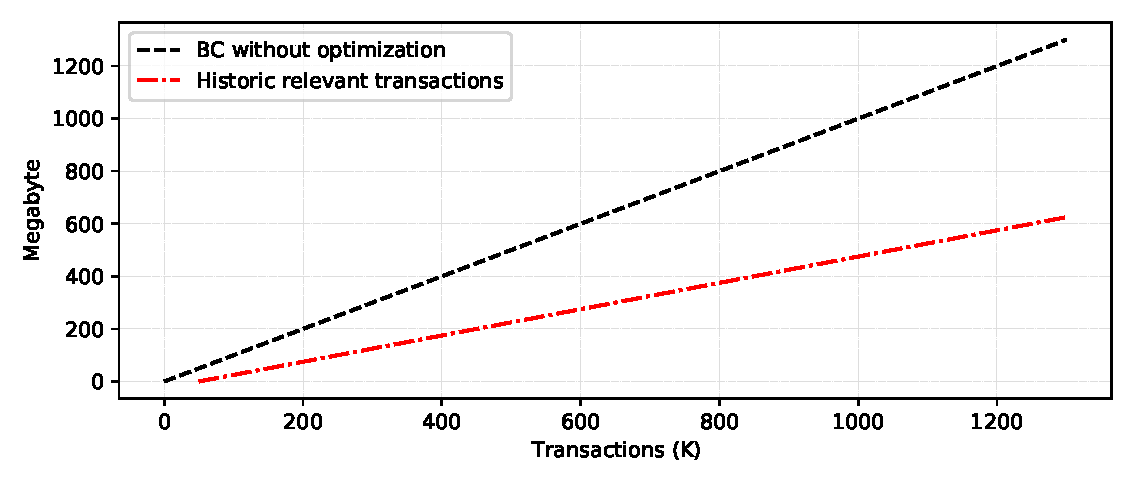
\includegraphics[width=.95\linewidth,keepaspectratio=true]{contents/images/BCstorageAllocationBase}
		\caption{General \gls{BT} storage allocation chart}
		\label{fig:StorageAllocation_Base}
	}
\end{figure}

\noindent \textbf{First} of course each \gls{BC} starts with a \hyperref[def_GenesisBlock]{genesis block} at 'zero'.
The displaced start of the two graphs
(Figure \ref{fig:StorageAllocation_Base}\footnote{\hspace{0.1cm}Figure \ref{fig:StorageAllocation_Base} plot's Python code is given in the \hyperref[script:GeneralStorageAllocation]{appendix}.}) reflects the \textit{offset revelation},
as unrevealed transactions can not be distinguished upon being \textit{historically relevant} or \textit{deletable}.
Accordingly to the predefined \textit{ratio}, the upper $\sim50$\% of the \gls{BC}'s size (Figure \ref{fig:StorageAllocation_Base}, '\gls{BC} without optimization')
accounts for \gls{BT}s (Figure \ref{fig:StorageAllocation_Base}, Area between the lines).
Nevertheless, only the '\textit{Historic relevant Transactions}' are needed long term (Figure \ref{fig:StorageAllocation_Base}, Lower line). \\
Estimating an average block to be of $\sim0.001$ MB and an active \gls{BC} to consist of $\sim100,000$ transactions,
it would consume $\sim100$ MB of storage space (Table \ref{tbl:BloatblocksBlockchainSize}, Row 1).
Consequently, $600,000$ transactions $* 0.001$ MB $= 600$ MB (see Figure \ref{fig:StorageAllocation_Base}).
Considering that there is not only one game being played simultaneously, the needed storage space raises linearly (Table \ref{tbl:BloatblocksBlockchainSize}, Row 2). \\
Although a single block consumes little storage space, massively generated \gls{BT} raise the allocated storage space tremendously.
Importantly, each entire \gls{BC} is supposed to be stored on all network nodes.
Generally, \gls{BCT} is built upon networks with well equipped nodes regarding hardware.
In contrast, (casual) gamers might want to join using devices which do not offer much storage space, such as smartphones or handheld consoles.
Here a storage size consuming \gls{BC}s could be limited by (other) software restrictions.
In the worst case it may lead to a removal of the application/game by the gamer or even by any higher authority,
such as popular app stores\footnote{\hspace{0.1cm}E.g.: Apple 'App Store', Google 'Play Store', Epic Games Store and the Steam Store}. \\
Consequently, a mechanism to reduce long termed storage allocation is needed.
Still, the thought of orderly deleting data within \gls{BCT} is far from the usual approach,
such that \gls{BCT} is thought to prevent removal of any content in general.
\begin{table}
	\centering
	\begin{tabularx}{0.59\textwidth}{ l | c | c }
		& 1 Transaction & 100,000 Transactions \\ \hline
		1 \gls{BC} game & $0.001$ MB & $100$ MB \\ \hline
		10 \gls{BC} games & $0.01$ MB & $1$ GB \\
		\hline
	\end{tabularx}
	\caption{Blockchain Size}
	\label{tbl:BloatblocksBlockchainSize}
\end{table}
Nevertheless, some approaches exists which make "[...] it possible to re-write or compress the content of any number of blocks in decentralized services [...]" \cite[111]{Ateniese.2017}.
These approaches are not considered in the scope of this thesis as they (only) \textit{compress} but do not \textit{delete} content.
Additionally, most \gls{BC}s prohibit deleting single transactions passively, as they are encapsulated in one block with other still needed transactions.
But in this special case of utilizing \gls{BT}s, the following three mechanisms could be identified to reduce allocated storage space:
\hyperref[sec:PruneProcedure]{Prune bloat transactions}, \hyperref[sec:CcTransition]{Child-chain transition}
(alike \citet{Kraft.2016}'s game channels) and \hyperref[sec:MeatState]{Meta-State Blocks}.


 
 \subsection{Prune bloat transactions}
 \label{sec:PruneProcedure}	
 Once a critical chain size is met, the chain could be recalculated using a \textbf{prune procedure}.
 As \textit{bloat transactions} could not be found in the literature, the deletion of these transactions is missing as well. \\
 The chain before the recalculation consisting of
 \gls{rrTs} (Figure \ref{fig:BloatBlocksPruneFromOrigin}),
 \textbf{revealed \gls{BT}s} (Figure \ref{fig:BloatBlocksPruneFromOrigin}, r\gls{BT}s),
 \textit{unrevealed \gls{BT}s} (Figure \ref{fig:BloatBlocksPruneFromOrigin}, u\gls{BT}s) as well as other negligible meta transactions
 is called the \textbf{untidy chain} (Figure \ref{fig:BloatBlocksPruneFromOrigin}, Untidy chain).\\
 The \gls{BC}'s network wants to get rid of meaningless allocated storage space and decides by vote to 'garbage collect' \textit{revealed \gls{BT}s} .
 One node has to conduct the \textit{prune procedure} - probably the node which broke a given \textit{untidy chain} size limit by adding transactions.
 The node calculating the prune is called the \gls{GCN}.
  \begin{figure}
 	\centering{
 		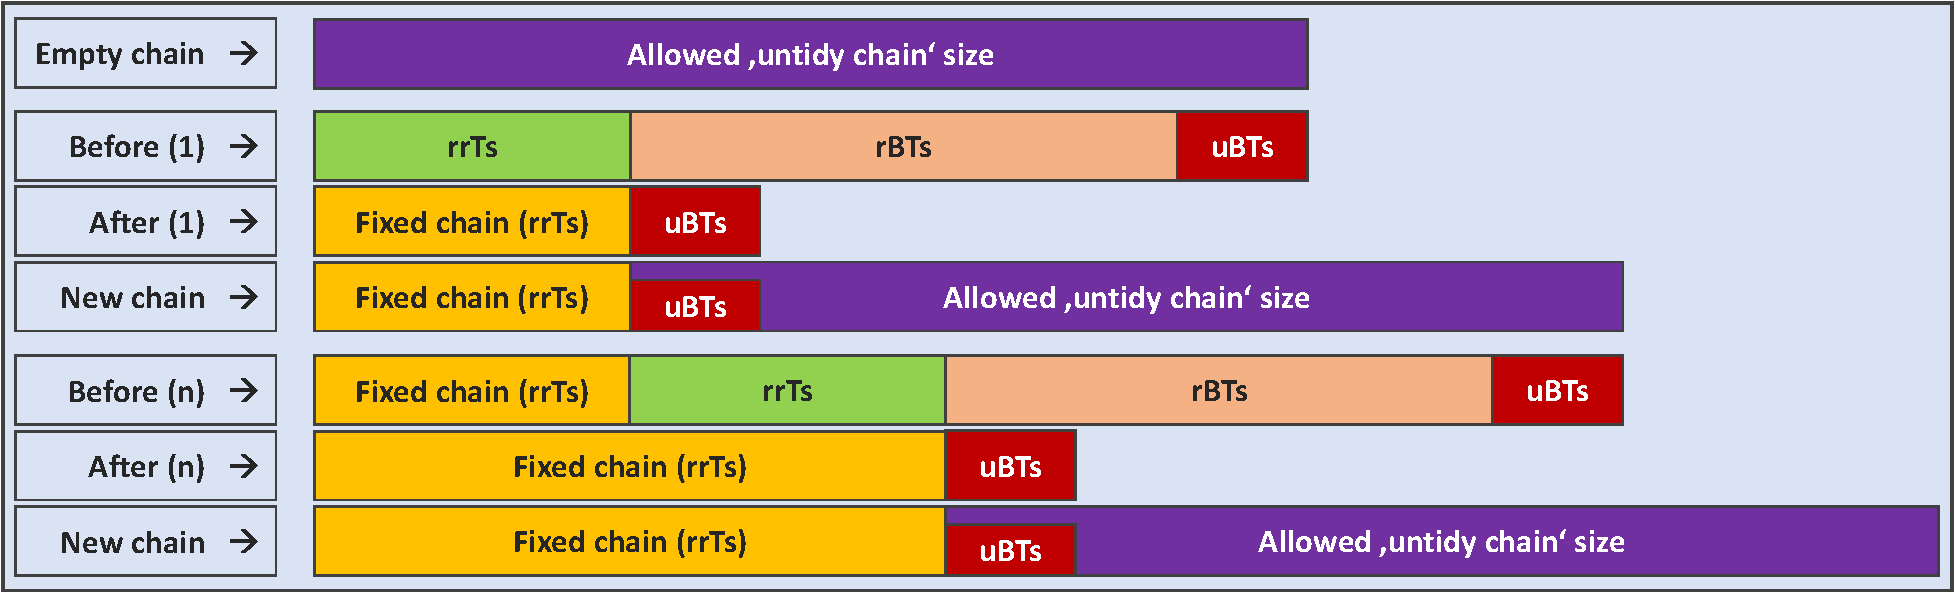
\includegraphics[width=.95\linewidth,keepaspectratio=true]{contents/images/BloatBlocksPruneFromOrigin}
 		\caption{Prune bloat transactions}
 		\label{fig:BloatBlocksPruneFromOrigin}
 	}
 \end{figure}

\noindent As \gls{rrTs}, \textit{revealed \gls{BT}s} and \textit{unrevealed \gls{BT}s}
are not separated or sorted within the \textit{untidy chain}, the \gls{GCN} generates a new chain from scratch except the \textbf{genesis block}.
During the recompilation, the \textit{untidy chain} is parsed by the \gls{GCN} and all \textit{revealed \gls{BT}s}
are deleted (Figure \ref{fig:BloatBlocksPruneFromOrigin}, Before(1) $\to$ After(1)).
This is only recommended in lightweight \gls{CM}s, as the \gls{GCN} needs to find suitable hashes for new blocks easily. 
Once the process is finished, another 'consensus vote' approves the new chain. \\
It has to be reminded that every network node exhibits the following behavior:
\begin{enumerate}
	\item Network nodes do not trust each other.
	The new chain, which was generated by the \gls{GCN} is checked/recalculated by every other network node.
	
	\item All network nodes have a desire to reduce their allocated storage space and look
	forward to a reduced chain - as long as the new chain complies with \textbf{one}.
\end{enumerate}
Consequently, if the \gls{GCN} fails to generate a valid new chain, the network tries to calculate a new chain delivered by another \gls{GCN}.
in this case, the first \gls{GCN} does not only have to calculate the first version, it also has to verify the second version.
Therefore every \gls{GCN} wants to avoid this (overhead workload) loose-loose situation which leads to honest recalculation and trust within the network. \\
The \gls{rrTs} are transitioned into a \textit{fixed chain} which will not be changed anymore (Figure \ref{fig:BloatBlocksPruneFromOrigin}, After (1): Fixed chain).
Transactions in the \textit{fixed chain} are unencrypted and do not store any additional bloat/coverage data.
Subsequent calculated \textit{prune procedures} will only focus on the 'new' \textit{untidy chain} (Figure \ref{fig:BloatBlocksPruneFromOrigin}, New chain: untidy chain).
Additionally, the \textit{untidy chain} size starts after the last \gls{rrTs} and directly contains all transactions which are not yet revealed. \\
All \gls{rrTs} which are transitioned into the fixed chain during this \textit{prune procedure}
may be written into a single block and signed by the \gls{GCN}, the transcribed encapsulated transactions are still signed by their emitting nodes.
Hence, the integrity of the chain is sustained.
Depending on the share of garbage data (\gls{BT}s/relevant transaction), the chain can be boiled down.
At the end of the \textit{prune procedure}, a marker is set which defines the start of the \textit{untidy chain}.
The next \textit{prune procedure} will start from that block (Figure \ref{fig:BloatBlocksPruneFromOrigin}, Before(n)). \\
Although the permanent growth of the \gls{BC} along '\textit{Historic relevant Blocks}'
(Figure \ref{fig:StorageAllocationPrune}\footnote{\hspace{0.1cm}Figure \ref{fig:StorageAllocationPrune}
	plot's Python code is given in the \hyperref[script:StorageAllocationPPSC]{appendix}.}, lower line)
can not be prevented using \textit{prune procedures} (Figure \ref{fig:StorageAllocationPrune}, Serrated line), the overall storage allocation can be dropped significantly. \\
If not triggered regularly, the prune approach is a computation heavy bulk operation.
It is computation heavy in the means of two factors:
\textbf{First}, generating the new chain as well as checking the integrity and \textbf{second}, in regards of network traffic to pass the whole new chain.
During a prune is calculated the game may be paused as described in section \hyperref[sec:PeerFluctuation]{Adaptive turn time} of the \hyperref[chap:PoT]{Proof-Of-Turn}.
Last, finding an optimal \textit{prune procedure} frequency (allocation size) is not part of this document.
For a more continuous approach to reduce allocated storage space, \textbf{Child-chain transitions} may be used.



\subsection{Child-chain transition}
\label{sec:CcTransition}
The idea of \textbf{child-chain transition} derives from \citet{Kraft.2016}'s \textit{game channels}.
Still, although \textit{game channels} conduct off-chain transactions using sidechains,
their intention is to speed up the main chain's throughput.
To the writers knowledge these \textit{game channels} are kept long term by the consulting parties.
Therefore, \textit{game channels} are not used for storage allocation improvements.
There was no further literature found regarding \textbf{child-chain transitions} for storage allocation improvements.
\begin{figure}[!b]
	\centering{
		\includegraphics[width=.95\linewidth,keepaspectratio=true]{contents/images/StorageAllocationPruneSC}
		\caption{Prune procedure/Child-chain chart}
		\label{fig:StorageAllocationPrune}
	}
\end{figure}

\noindent A downside of \textit{prune procedures} is the aforementioned peak of computation and network traffic on one single node.
A continuous \textbf{child-chain transition} from \textit{child-chains}
(see \hyperref[sec:PerformanceImprovements]{Performance Improvements})
to the \textit{main-chain} may be a reasonable answer to this challenge.
Here, a game uses an undefined number of \textit{child-chains} (Figure \ref{fig:BloatBlocksChildChain}),
each limited to e.g. $1$ MB ($\sim 1000$ transactions, following Table \ref{tbl:BloatblocksBlockchainSize}). \\
Whilst the \textbf{main-chain} stores all \gls{rrTs}, all unrevealed transactions are stored in \textit{child-chains}.
Once the storage size of a \textit{child-chain} is exceeded, all newly published blocks will be stored
on the next \textit{child-chain} (Figure \ref{fig:BloatBlocksChildChain}, \textit{n} $\to$ \textit{n+1}).
The newest \textit{child-chains} may therefore consist of \textit{unrevealed \gls{BT}s} only (Figure \ref{fig:BloatBlocksChildChain}, \textit{n+1}).
Still the filled \textit{child-chains} are temporarily kept (Figure \ref{fig:BloatBlocksChildChain}, \textit{1}, \textit{n-1} and \textit{n}). \\
By the time a transaction is revealed, the revelation key will be put on the dedicated \textit{child-chain}
- next to the unrevealed transaction - and the unencrypted residue is stored on the \textit{main-chain}.
Hence the \textit{main-chain} is unencrypted throughout.
\begin{figure}
	\centering{
		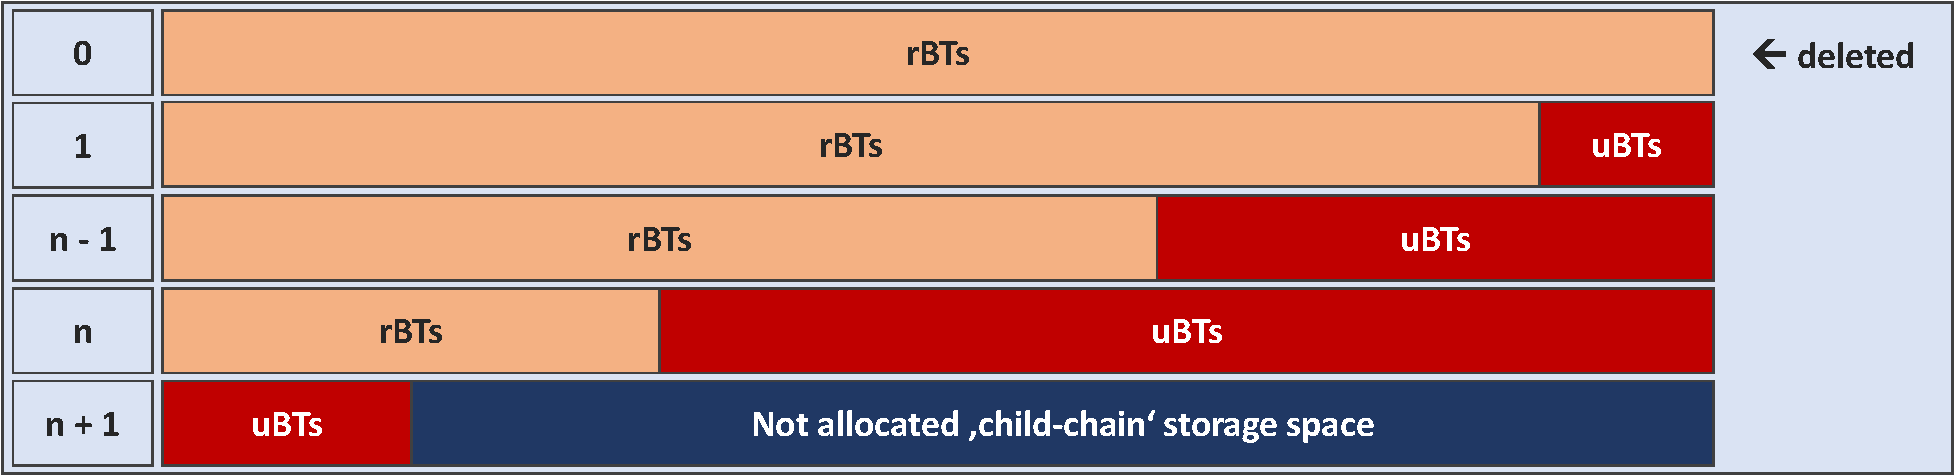
\includegraphics[width=.95\linewidth,keepaspectratio=true]{contents/images/BloatBlocksChildChain}
		\caption{Child-chain storage allocation}
		\label{fig:BloatBlocksChildChain}
	}
\end{figure}

\noindent By the time all transactions on a \textit{child-chain} are revealed or obsolete, the \textit{child-chain} can be deleted (Figure \ref{fig:BloatBlocksPruneFromOrigin}, 0).
The deletion is conducted by each node individually.
Hence a node - if desired - could keep the data as well.
Concluding, bloat/coverage data, which has initially been added to \gls{rrTs} becomes obsolete and
the key emitting (/revealing) node itself can sign the blocks on the \textit{main-chain} as well.
In this scenario \textit{child-chains} with small storage sizes offer faster deletion as it has to be waited until the last transaction is revealed.
Nevertheless, although small storage sizes lead to smooth overall storage allocation,
more filled \textit{child-chains} have to be stored until they can be deleted. \\
The overall storage size equals to the one from \textit{prune procedures} (Figure \ref{fig:StorageAllocationPrune}, Serrated line).
In this regards, frequent \textit{prune procedures} and small \textit{child-chains} equal each other as
seldom \textit{prune procedures} and big \textit{child-chains} do.
Whilst \textit{child-chains} offer an comparably equal distribution of computation and network traffic,
\textit{prune procedures} could be designed to be conducted on nodes offering strong computation power only. \\
Still, for \textit{child-chains} a lightweight \gls{CM} is needed throughout.
Finding an optimal \textit{child-chain} size is not part of this document.



\subsection{Meta-State Blocks}
\label{sec:MeatState}
Both, the \textit{prune procedure}- as well as the \textit{child-chain}-approach offer a full (game) history.
Nevertheless, if storage space is limited, the network could decide to define any fully
\begin{figure}[!b]
	\centering{
		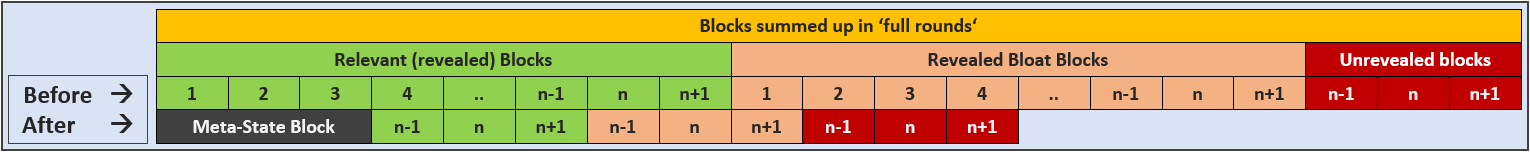
\includegraphics[width=.95\linewidth,keepaspectratio=true]{contents/images/BloatBlocksMetaState}
		\caption{Meta-State Block process step}
		\label{fig:BloatBlocksMetaState}
	}
\end{figure}
revealed state - before the first \textit{unrevealed (bloat) transaction} - to be the new \textbf{genesis} (block).
Again there was no literature found which changes the genesis block to rewrite a \gls{BC}'s history for data allocation improvements. \\
A new \textbf{meta-state block}, at the beginning of the chain, represents the game's state at the \textit{genesis}
(Figure \ref{fig:BloatBlocksMetaState}, \textit{After}: Meta-State Block).
The \textit{meta-state block} summarizes all until then emitted transactions, defining a 'new default start'.
Old obsolete transactions are dropped, obfuscating 'historical relevant' data (Figure \ref{fig:StorageAllocation_MetaState}\footnote{\hspace{0.1cm}Figure \ref{fig:StorageAllocation_MetaState} plot's Python code is given in the \hyperref[script:StorageAllocationMetaState]{appendix}.}, Meta-State Block).
Except historically relevant values, the data in the \textit{meta-state block} does not differ from the network's knowledge 'at the starting point' (Figure \ref{fig:BloatBlocksMetaState}, \textit{Before}: '..|' $\to$ \textit{After}: Meta-State Block).
Therefore, it is encouraged not to use the last unrevealed (bloat) transaction, but to leave some historic data in between (Figure \ref{fig:BloatBlocksMetaState}, \textit{After}: 'n-2' $\to$ 'n', 'o-2' $\to$ 'o' and 'p-2' $\to$ 'p').
\begin{figure}
	\centering{
		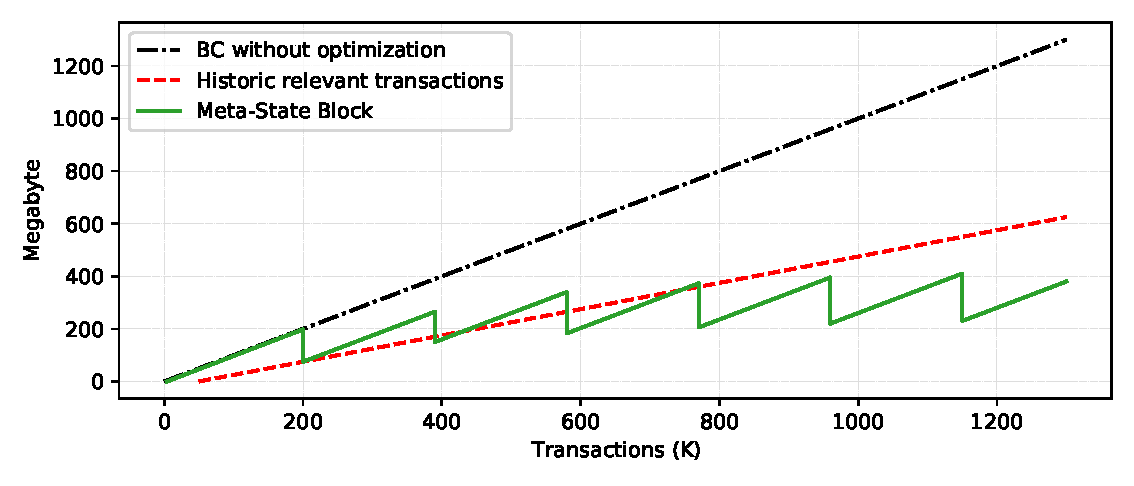
\includegraphics[width=.95\linewidth,keepaspectratio=true]{contents/images/storageAllocationMetaState}
		\caption{Meta-State Block chart}
		\label{fig:StorageAllocation_MetaState}
	}
\end{figure}

\noindent Although it is discouraged from, the equivalent in a cryptocurrency context would be
a \textit{meta-state block} at the beginning of (e.g.) the last elapsed
year - the wallets amounts remain the same, but transactions before
the \textit{meta-state block} can not be retrieved anymore.
Still, each node is free to either \textit{keep} or \textit{delete} the until then generated (old) chain.
Nevertheless, here it is assumed that the described nodes drop the old chain and receive
released allocated storage space in exchange (Figure \ref{fig:StorageAllocation_MetaState}, Meta-State Block).
\begin{figure}[!b]
	\centering{
		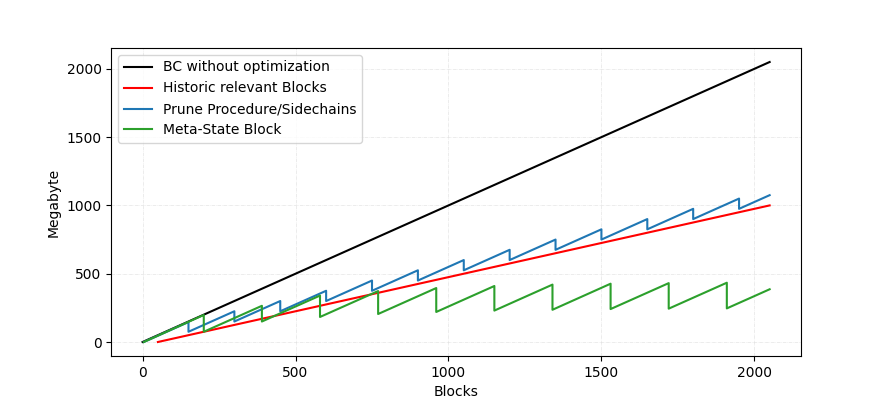
\includegraphics[width=.95\linewidth,keepaspectratio=true]{contents/images/BCstorageAllocationAllBig}
		\caption{Storage allocation comparison}
		\label{fig:BC_StorageAllocation_All_Big}
	}
\end{figure}

\noindent Consequenly, in contrast to \textit{prune procedures} and \textit{child-chains}, all previous \textit{meta-state blocks}
containing movement information, randomization agreements and other transactions are deleted.
The \textit{meta-state block} is always the genesis.
Agreeing to the trade-off, the network looses its history before the genesis round, but retrieves storage space (Figure \ref{fig:StorageAllocation_MetaState}, Meta-State Block).
The baseline after the historic data was deleted was set to sample $\sim200$MB long term (Figure \ref{fig:StorageAllocation_MetaState}). \\
In figure \ref{fig:StorageAllocation_MetaState} it is assumed, that the application allocates an equal amount of storage in the long run, e.g. $\geq1.000k$ transactions.
Until this level is reached, the \textit{meta-state block}-approach is (here) not especially advantageous.
Given a (smaller) larger transactions size, this metric changes.
This method is well suited for applications, wherein history is considered obsolete in general.
Still all \gls{SC}s need to remain consistent for the upper level software.
Although the \textit{meta-state block}-approach is mentioned independently,
it can be combined with both, the \textit{prune procedure}- as well as the \textit{child-chain}-approach. \\
Finally, figure \ref{fig:BC_StorageAllocation_All_Big}\footnote{\hspace{0.1cm}Figure \ref{fig:BC_StorageAllocation_All_Big} plot's Python code is given in the \hyperref[script:StorageAllocationComp]{appendix}.}
shows the procedures together in one plot in larger scale ($2.000k$ transactions).
All procedures combine the characteristic that cheating is not possible, because only those blocks which are already verified by the network are deleted.
Of course, systems which contain 'above-average storage space' are able to keep historic data (longer).
Nevertheless, superior systems do not have any advantage regarding the quality of the stored information or benefits regarding upper level game play.



\section{Interim Summary - Blockchain Technology in Games}
\label{sec:InterimSummary-BCTinG}
Before presenting the \gls{PoT} \gls{CM}, a short summary of the so far identified results is given.
This chapter shows that \gls{BCT} is suitable for certain \hyperref[sec:GamingMarket]{games}
(e.g. \textit{gambling} and \textit{collectibles}) and is in some regards
already used to enable new types of games (here: \textit{collectibles}).
Still, publishers do not yet use \gls{BCT} to reduce network costs but rather
try to leverage cryptocurrencies and assets backed by \gls{NFTs} to boost their revenue.
Further, these applications proof that recent \gls{CM}s are already able to host slow games generally. \\
Additionally, a \hyperref[sec:ProblemSpace]{problem space} was defined to identify general, primarily board game related, \gls{SC}s.
Thereafter, \hyperref[sec:HiddenTransactionsPlusRandomization]{Hidden transactions \& Randomization},
\hyperref[sec:PileOfCards]{Piles of Cards}, \hyperref[sec:FogOfWar]{Fog of War}, as well as 
\hyperref[sec:RcTeDisputes]{Reveal claims, trigger events \& Disputes} were analyzed.
Last, possible \hyperref[sec:DataAllocationImprovements]{Data allocation improvements},
new to \gls{BCT}, were presented. \\
All these \gls{SC}s were given to answer the guiding question:
\begin{center}
	\textit{"Which kind of \gls{SC}s need to be established to cover typical in-game mechanics?"}
\end{center}
In this regards, one key factor has to be mentioned again:
A game can only be won by offering a full disclosure of all hidden content.
Without this final revelation it has to be assumed that fraud is being covered and
consequently the affected node is not allowed to win. \\

\noindent Nevertheless, the section covering the \hyperref[sec:GamingMarket]{Gaming market}
emphasizes the importance of well performing games on mobile devices such as smartphones.
Looking at the recent storage capacity of smartphones, \gls{BCT} games
developed for mobile devices probably demand the just described
\hyperref[sec:DataAllocationImprovements]{Data allocation improvements} to reach reasonable customer bases.
But the aforementioned \gls{CM}s do not offer the mandatory characteristic
to grant lightweight writing permission freely to specific nodes, whilst
keeping an adjustable \gls{BFT} - especially in the \textit{proof-of} category. \\
Therefore, a \gls{CM} offering these characteristics to enable games
on mobile operating systems, such as Google's Android and Apple's iOS is seen crucial
for \gls{BCT} to evolve further applications and use cases.
Additionally it would prevent the need for \textit{nerdy peer} setting up dedicated servers
and circumvent the \textit{shadow server} problem.
Last, the comparably easy option of providing updates to the gamer's devices via the app stores
reduces the publishers constraints to gamers not willing to update their dedicated servers to recent changes. \\
Consequently, next the \hyperref[chap:PoT]{Proof-of-Turn} algorithm is presented.


